\documentclass[sigconf]{acmart}

\usepackage{booktabs}
\usepackage{setspace}
\usepackage{listings}
\usepackage{courier}
\usepackage{enumitem}
\usepackage{multirow}
\usepackage{color}
\usepackage{xcolor}
\usepackage{totpages}

  \let\oldthebibliography=\thebibliography
  \let\endoldthebibliography=\endthebibliography
  \renewenvironment{thebibliography}[1]{%
    \begin{oldthebibliography}{#1}%
      \setlength{\parskip}{0ex}%
      \setlength{\itemsep}{0ex}%
  }%
  {%
    \end{oldthebibliography}%
  }


\sloppy
%
% Generic Defines
%

\newcommand{\mm}{mm$^2$}
\newcommand{\figtitle}[1]{\textbf{#1}}
\newcommand{\us}{$\mu$s}
\newcommand{\fixme}[1]{{\color{red}\textbf{\fbox{FIXME} #1}}}
\newcommand{\FIXME}[1]{{\color{red}\textbf{\fbox{FIXME} #1}}}
\newcommand{\TODO}[1]{{\color{red}\textbf{\fbox{TODO} #1}}}
\newcommand{\NOTE}[1]{{\color{blue}\textbf{\fbox{NOTE} #1}}}
\newcommand{\note}[1]{{\color{blue}\textbf{\fbox{NOTE} #1}}}

\newcommand{\yiying}[1]{{\color{cyan}\textbf{\fbox{Yiying} #1}}}
\newcommand{\arvind}[1]{{\color{orange}\textbf{\fbox{Arvind} #1}}}
\newcommand{\yizhou}[1]{{\color{red}\textbf{\fbox{Yizhou} #1}}}
\newcommand{\ryan}[1]{{\color{green}\textbf{\fbox{Ryan} #1}}}
\newcommand{\will}[1]{{\color{olive}\textbf{\fbox{Will} #1}}}
%\fbox{Zac} #1}}}

%\newcommand{\note}[2]{\fixme{$\ll$ #1 $\gg$ #2}}

\newcommand{\myitem}[1]{\item \textbf{#1}}
\newcommand{\myitemit}[1]{\item \textit{#1}}
\newcommand{\horizbar}{\rule{\linewidth}{.5mm}}
\newcommand{\app}[1]{{\sc #1}}
 
\renewcommand{\em}{\it}

  
\newcommand{\BigO}[1]{${\cal O}(#1)$}
\newcommand{\BigOmega}[1]{$\Omega(#1)$}
\newcommand{\BigTheta}[1]{$\Theta(#1)$}
 
\newcommand{\ceiling}[1]{\left\lceil #1 \right\rceil}
\newcommand{\faM}{\lfloor \alpha M \rfloor}
%\newcommand{\C}[2]{{#1 \choose #2}}

\newcommand{\x}{$\times$}
 
%\newcommand{\comment}[1]{}
\newcommand{\ignore}[1]{}


%\newcommand{\boldparagraph}[1]{\vspace*{-0ex}\paragraph{#1}}
\newcommand{\boldparagraph}[1]{\vspace*{1ex}\noindent\textit{#1}\hspace{1em}}

%%%%% SINGLE FIGURE
\def\cfigure[#1,#2,#3]{
\begin{figure}
\vspace*{0mm}
\begin{center}

\includegraphics[width=3in]{#1} 
 
\vspace*{-3mm}\caption[]{#2
} \label{#3}
 
\vspace*{-5mm}
\end{center}
%\horizbar
%\vspace*{-2mm}
\end{figure}}

%%%%% SINGLE FIGURE 4in wide
\def\cfigurefour[#1,#2,#3]{
\begin{figure}
\vspace*{0mm}
\begin{center}

\includegraphics[width=4in]{#1} 
 
\vspace*{-3mm}\caption[]{#2
} \label{#3}
 
\vspace*{-5mm}
\end{center}
%\horizbar
%\vspace*{-2mm}
\end{figure}}

%%%%% SINGLE FIGURE
\def\cfiguretemp[#1,#2,#3]{
\begin{figure}
\vspace*{0mm}
\begin{center}

\includegraphics[width=3.5in]{#1} 
 
\vspace*{-3mm}\caption[]{#2
} \label{#3}
 
\vspace*{-5mm}
\end{center}
%\horizbar
\vspace*{-2mm}
\end{figure}}

%%%%% SINGLE WIDE FIGURE
\def\wfigure[#1,#2,#3]{
\begin{figure*}
\vspace*{0mm}
\begin{center}
 \includegraphics[width=\textwidth]{#1} 
 \vspace*{-3mm}\caption[]{#2
} \label{#3}
 
\end{center}
%\horizbar
\end{figure*}}

%%%%% 3 FIGURES IN A ROW
\def\threefigure[#1,#2,#3,#4,#5]{
\begin{figure*}
\vspace*{0mm}
\begin{center}

\begin{tabular}{ccc}
\includegraphics[width=2in]{#1} & \includegraphics[width=2in]{#2} &  \includegraphics[width=2in]{#3} \\
(a) & (b) & (c) \\
\end{tabular}

\vspace*{-3mm}\caption[]{#4
} \label{#5}

\vspace*{-5mm}
\end{center}
%\horizbar
\vspace*{-2mm}
\end{figure*}}

%%%%%% DOUBLE FIGURE
\def\dcfigure[#1,#2,#3,#4,#5,#6]{
{
\begin{figure*}
\begin{center}
\begin{minipage}[c]{\columnwidth}{
\includegraphics[width=\columnwidth]{#1} 
\vspace*{0mm}\caption[]{#2} \label{#3} \
}\end{minipage}\hspace*{\columnsep}\
\begin{minipage}[c]{\columnwidth}{
\includegraphics[width=\columnwidth]{#4} 
\vspace*{0mm}\caption[]{#5}\label{#6} \
}\end{minipage}
\end{center}
\end{figure*}
}
}


\def\tableByTable[#1,#2,#3,#4,#5,#6]{
{
\begin{table*}
\begin{center}
\begin{minipage}[c]{3in}{
\centering
{#1}
\vspace*{0mm}\tabcaption[]{#2}\label{#3} \
}\end{minipage}\hspace*{\columnsep}\
\begin{minipage}[c]{3in}{
\centering
{#4}
\vspace*{0mm}\tabcaption[]{#5}\label{#6} \
}\end{minipage}
\end{center}
\end{table*}
}
}


\def\figureByTable[#1,#2,#3,#4,#5,#6]{
{
\begin{figure*}
\begin{center}
\begin{minipage}[c]{3in}{
\centering
\includegraphics[width=\textwidth]{#1}
\vspace*{0mm}\figcaption[]{#2} \label{#3} \
}\end{minipage}\hspace*{\columnsep}\
\begin{minipage}[c]{3.3in}{
\centering
{#4}
\vspace*{0mm}\tabcaption[]{#5}\label{#6} \
}\end{minipage}
\end{center}
\end{figure*}
}
}

\def\tableByFigure[#1,#2,#3,#4,#5,#6]{
{
\begin{figure*}
\begin{center}
\begin{minipage}[c]{4.3in}{
\centering
{#1}
\vspace*{0mm}\tabcaption[]{#2} \label{#3} \
}\end{minipage}\hspace*{\columnsep}\
\begin{minipage}[c]{2.2in}{
\centering
\includegraphics[width=\textwidth]{#4}
\vspace*{-0.35in}\caption[]{#5}\label{#6} \
}\end{minipage}
\end{center}
\end{figure*}
}
}

% two figs pdfs in one column fig
\def\doublecfigure[#1,#2,#3,#4]{
{
\begin{figure}
\begin{center}
\begin{minipage}[c]{1.5in}{
\begin{center}
\includegraphics[width=1.5in]{#1}%\\(a)
\end{center}
}\end{minipage}\hspace*{1em}\
\begin{minipage}[c]{1.5in}{
\begin{center}
\includegraphics[width=1.5in]{#2}%\\(b)
\end{center}
}\end{minipage}
\vspace*{0mm}\caption[]{#3} \label{#4} \
\end{center}
\end{figure}
}
}

\def\qcfigure[#1,#2,#3,#4,#5,#6]{
{
\begin{figure*}
\vspace*{0.2in}\
\begin{center}
\begin{minipage}[c]{3in}{
\includegraphics[width=3in]{#1} 
\vspace*{-3mm}
}
\end{minipage}\hspace*{0.5in}\
\begin{minipage}[c]{3in}{
\includegraphics[width=3in]{#2} 
\vspace*{-3mm}
}\end{minipage}

\begin{minipage}[c]{3in}{
\includegraphics[width=3in]{#3} 
\vspace*{-3mm}
}
\end{minipage}\hspace*{0.5in}\
\begin{minipage}[c]{3in}{
\includegraphics[width=3in]{#4} 
\vspace*{-3mm}
}\end{minipage}
\end{center}
\caption[]{#5}\label{#6}
\end{figure*}
}
}

\def\twfigure[#1,#2,#3,#4,#5]{
{
\begin{figure*}
\vspace*{0.2in}\
\begin{center}
\begin{minipage}[c]{6.5in}{
\includegraphics[width=6.5in]{#1} 
\vspace*{-3mm}
}
\end{minipage}

\begin{minipage}[c]{6.5in}{
\includegraphics[width=6.5in]{#2} 
\vspace*{-3mm}
}\end{minipage}

\begin{minipage}[c]{6.5in}{
\includegraphics[width=6.5in]{#3} 
\vspace*{-3mm}
}
\end{minipage}
\end{center}
\caption[]{#4}\label{#5}
\end{figure*}
}
}

\def\dwfigure[#1,#2,#3,#4]{
{
\begin{figure*}
\vspace*{0.2in}\
\begin{center}
\begin{minipage}[c]{6.5in}{
\includegraphics[width=6.5in]{#1} 
\vspace*{-3mm}
}
\end{minipage}

\begin{minipage}[c]{6.5in}{
\includegraphics[width=6.5in]{#2} 
\vspace*{-3mm}
}\end{minipage}

\end{center}
\caption[]{#3}\label{#4}
\end{figure*}
}
}



\def\dssfigure[#1,#2,#3,#4,#5,#6]{
{
\begin{figure*}
\vspace*{0.2in}\
\begin{center}
\begin{minipage}[c]{4in}{
\includegraphics[width=4in]{#1}
\vspace*{-3mm}\caption[]{#2} \label{#3} \
}\end{minipage}\hspace*{0.5in}\
\begin{minipage}[c]{2in}{
\includegraphics[width=2in]{#4}
\vspace*{-3mm}\caption[]{#5}\label{#6} \
}\end{minipage}
\end{center}
\vspace*{-0.4in}\
\end{figure*}
}
}




\def\dsfigure[#1,#2,#3,#4,#5,#6]{
{
\begin{figure*}
\vspace*{0.2in}\
\begin{center}
\begin{minipage}[c]{3in}{
\includegraphics[width=3in]{#1}
\vspace*{-3mm}\caption[]{#2} \label{#3} \
}\end{minipage}\hspace*{0.5in}\
\begin{minipage}[c]{3in}{
\hspace*{0.5in}\
\includegraphics[height=3in]{#4}
\vspace*{-3mm}\caption[]{#5}\label{#6} \
}\end{minipage}
\end{center}
\vspace*{-0.4in}\
\end{figure*}
}
}


\def\dsyfigure[#1,#2,#3,#4,#5,#6]{
{
\begin{figure*}
\vspace*{0.2in}\
\begin{center}
\begin{minipage}[c]{2.5in}{
\includegraphics[height=2.5in]{#1}
\vspace*{-3mm}\caption[]{#2} \label{#3} \
}\end{minipage}\hspace*{0.5in}\
\begin{minipage}[c]{2.5in}{
\includegraphics[height=2.5in]{#4}
\vspace*{-3mm}\caption[]{#5}\label{#6} \
}\end{minipage}
\end{center}
\vspace*{-0.4in}\
\end{figure*}
}
}

\def\dyfigure[#1,#2,#3,#4,#5,#6]{
{
\begin{figure*}
\vspace*{0.2in}\
\begin{center}
\begin{minipage}[c]{3in}{
\includegraphics[height=3in]{#1} 
\vspace*{-3mm}\caption[]{#2} \label{#3} \
}\end{minipage}\hspace*{0.5in}\
\begin{minipage}[c]{3in}{
\includegraphics[height=3in]{#4} 
\vspace*{-3mm}\caption[]{#5}\label{#6} \
}\end{minipage}
\end{center}
\vspace*{-0.4in}\
\end{figure*}
}
}

%%%%%% DOUBLE FIGURE Y
\def\dyoldfigure[#1,#2,#3,#4,#5,#6]{
{
\begin{figure*}
\vspace*{0.2in}\
\begin{center}
\begin{minipage}[c]{3in}{
\epsfysize=2.0in\
\hspace{0.5in}\
\epsfbox{#1}
\vspace*{-3mm}\caption[]{#2} \label{#3} \
}\end{minipage}\hspace*{0.25in}\
\begin{minipage}[c]{3in}{
\epsfysize=2.0in\
\hspace{0.5in}\
\epsfbox{#4}
\vspace*{-3mm}\caption[]{#5}\label{#6} \
}\end{minipage}
\end{center}
\vspace*{-0.4in}\
\end{figure*}
}
}

%%%%%% DOUBLE FIGURE Y IN A COLUMN!!
\def\cfiguredouble[#1,#2,#3,#4]{
\begin{figure}
\vspace*{0.2in}\
\begin{center}
\begin{minipage}[c]{1.5in}{
\epsfxsize=1.5in\
\epsfbox{#1}
}\end{minipage}\hspace*{0.1in}\
\begin{minipage}[c]{1.5in}{
\epsfxsize=1.5in\
\vspace{0.1in}\epsfbox{#2}
}\end{minipage}\vspace*{-0.10in} \caption[]{#3}\label{#4}
\end{center}
\vspace*{-0.4in}\
\end{figure}
}


%%%%% Single programmable size figure
\def\wpfigure[#1,#2,#3,#4]{
\begin{figure*}
\vspace*{4mm}
\begin{center}

\includegraphics[width=#4]{#1} 

\vspace*{-3mm}\caption[]{#2
} \label{#3}

\vspace*{-5mm}
\end{center}
%\horizbar
\end{figure*}}

%%%%% Single programmable size figure, rotated
\def\wprfigure[#1,#2,#3,#4,#5]{
\begin{figure*}
\vspace*{4mm}
\begin{center}

\includegraphics[width=#4, angle=#5]{#1} 

\vspace*{-3mm}\caption[]{#2
} \label{#3}

\vspace*{-5mm}
\end{center}
%\horizbar
\end{figure*}}




%%%%% Adjacent, programmable-width figures, slid vertically by 9th
%%%%% parameter
\def\DoubleFigureWSlide[#1,#2,#3,#4,#5,#6,#7,#8,#9]{
\begin{figure*}
\vspace*{#9}
\begin{center}
\begin{minipage}{#4}
\includegraphics[width=#4]{#1}
\vspace*{-3mm}\caption{#2
}\label{#3}
\end{minipage}
\hspace{2em}
\begin{minipage}{#8}
\includegraphics[width=#8]{#5}
\vspace*{-3mm}\caption{#6
}\label{#7}
\end{minipage}
\vspace*{-5mm}
\end{center}
\end{figure*}
}


%%%%% Adjacent, programmable-width figures
\def\DoubleFigureW[#1,#2,#3,#4,#5,#6,#7,#8]{
\begin{figure*}
\vspace*{0in}
\begin{center}
\begin{minipage}{#4}
\includegraphics[width=#4]{#1}
\vspace*{-3mm}\caption{#2
}\label{#3}
\end{minipage}
\hspace{2em}
\begin{minipage}{#8}
\includegraphics[width=#8]{#5}
\vspace*{-3mm}\caption{#6
}\label{#7}
\end{minipage}
\vspace*{-5mm}
\end{center}
\end{figure*}
}



\def\DoubleFigureWHack[#1,#2,#3,#4,#5,#6,#7,#8]{
\begin{figure*}
\vspace*{0in}
\begin{center}
\begin{minipage}{3in}
\includegraphics[width=#4]{#1}
\vspace*{-3mm}\caption{#2
}\label{#3}
\end{minipage}
\hspace{2em}
\begin{minipage}{3in}
\includegraphics[width=#8]{#5}
\vspace*{-3mm}\caption{#6
}\label{#7}
\end{minipage}
\vspace*{-5mm}
\end{center}
\end{figure*}
}






%%%%%% DOUBLE FIGURE
\def\ddcfigure[#1,#2,#3,#4]{
\begin{figure*}
\vspace*{0.2in}\
\begin{center}
\begin{minipage}[c]{\columnwidth}{
\includegraphics[width=\columnwidth]{#1} 
}\end{minipage}\hspace{0.5in}\
\begin{minipage}[c]{\columnwidth}{
\includegraphics[width=\columnwidth]{#2} 
}\end{minipage} \caption[]{#3}\label{#4}
\end{center}
\end{figure*}
}

\def\ddcfigureSlide[#1,#2,#3,#4,#5]{
\begin{figure*}
\vspace*{#5}\
\begin{center}
\begin{minipage}[c]{3in}{
\includegraphics[height=3in]{#1} 
}\end{minipage}\hspace{0.5in}\
\begin{minipage}[c]{3in}{
\includegraphics[height=3in]{#2} 
}\end{minipage}\vspace*{-0.10in} \caption[]{#3}\label{#4}
\end{center}
\vspace*{-0.4in}\
\end{figure*}
}

\def\cxfigure[#1,#2,#3]{
\begin{figure}
\vspace*{4mm}
\begin{center}
 
\epsfxsize=2.5in\
\epsfbox{#1}\
 
\vspace*{-0.10in}\caption[]{#2
} \label{#3}
 
\vspace*{-5mm}
\end{center}
%\horizbar
\vspace*{-2mm}
\end{figure}}

\newenvironment{panefigure}{\begin{figure}\begin{center}}{\end{center}\end{figure}}

\newcommand{\pdfpane}[3]{
\begin{minipage}{#1}
\begin{center}
\includegraphics[width=#1]{#2}\\(#3)
\end{center}
\end{minipage}
}

\newcommand{\figWidth}{\columnwidth}
\newcommand{\figSep}{0.05in} 
%\newcommand{\figSep}{\columnsep} 
\newcommand{\figWidthOne}{3.05in} 
\newcommand{\figWidthHalf}{5.85in} 
\newcommand{\figWidthTwo}{3.7in} 
\newcommand{\figWidthThree}{2in} 
\newcommand{\figWidthFour}{1.3in} 
\newcommand{\figWidthFive}{2.3in} 
\newcommand{\figWidthSix}{2.3in} 
\newcommand{\figHeight}{2.0in}
\newcommand{\figHeightOne}{2.6in}
\newcommand{\captionText}[2]{\textbf{#1} \textit{\small{#2}}}

\newcommand{\beforecaption}{\vspace{-.15cm}\begin{spacing}{0.85}}
\newcommand{\aftercaption}{\vspace{-.45cm}\end{spacing}}
% \newcommand{\mycaption}[3]{{\beforecaption\caption{\label{#1}\footnotesize{\textbf{#2}} {\em #3}}\aftercaption}}
% haryadi, change mycaption three to mycaptionthree
%\newcommand{\mycaption}[3]{{\caption[#2]{{\bf #2.} {\em #3}}\label{#1}}}
%\newcommand{\mycaption}[3]{\beforecaption\caption{\label{#1}{\small \bf #2} \em\scriptsize #3}\aftercaption}
%\newcommand{\mycaption}[3]{\beforecaption\caption{\label{#1}{\bf #2} \em\footnotesize #3}\aftercaption}
\newcommand{\mycaption}[3]{\caption{\label{#1}{\bf #2} \em\small #3}}


%%%%% general

% only foreign words should be italicized... (example given should not)
\newcommand{\eg}{\textit{e.g.}}
\newcommand{\ie}{\textit{i.e.}}
\newcommand{\etal}{\textit{et al.}}
\newcommand{\etc}{\textit{etc.}}
\newcommand{\adhoc}{\textit{ad hoc}}

% units
\newcommand{\KB}{\,KB}
\newcommand{\MB}{\,MB}
\newcommand{\GB}{\,GB}
\newcommand{\TB}{\,TB}
\newcommand{\GBs}{\,GB/s}
\newcommand{\MBs}{\,MB/s}
\newcommand{\KBs}{\,KB/s}
\newcommand{\Kbs}{~Kbit/s}
\newcommand{\gbps}{\,Gbps}
\newcommand{\mbs}{~Mbit/s}
\newcommand{\mus}{\mbox{$\mu s$}}
\newcommand{\ms}{\mbox{$ms$}}

%\newcommand{\fsync}{\texttt{fsync}}

% axes
\newcommand{\xaxis}{x-axis}
\newcommand{\yaxis}{y-axis}


\newcommand{\unix}{{\sc Unix}}
\newcommand{\NULL}{{\sc NULL}}
\newcommand{\sysread}{\texttt{read}}
\newcommand{\syssync}{\texttt{sync}}
\newcommand{\fsync}{\texttt{fsync}}
\newcommand{\syswrite}{\texttt{write}}
\newcommand{\sysseek}{\texttt{lseek}}
\newcommand{\sysstat}{\texttt{stat}}
\newcommand{\make}{\texttt{make}}
\newcommand{\ioctl}{\texttt{ioctl}}
\newcommand{\panic}{\texttt{panic}}
\newcommand{\truncate}{\texttt{truncate}}
\newcommand{\rmdir}{\texttt{rmdir}}
\newcommand{\unlink}{\texttt{unlink}}
\newcommand{\open}{\textit{open}}
\newcommand{\close}{\textit{close}}
\newcommand{\linkscount}{\texttt{linkscount}}
\newcommand{\msync}{\textit{msync}}
\newcommand{\mmap}{\textit{mmap}}
\newcommand{\unmap}{\textit{munmap}}
\newcommand{\map}{\textit{map}}
\newcommand{\fetch}{\textit{gfetch}}
\newcommand{\acquire}{\textit{acquire}}
\newcommand{\commitxact}{\textit{commit}}
\newcommand{\commit}{\textit{commit}}
\newcommand{\barrier}{\textit{thread-barrier}}


% dsnvm
\newcommand{\dsnvm}{DSPM}
\newcommand{\dsm}{DSM}
\newcommand{\nvm}{PM}
\newcommand{\hotpot}{Hotpot}
\newcommand{\mrmw}{MRMW}
\newcommand{\mrsw}{MRSW}
\newcommand{\wfetch}{FETCH}
\newcommand{\cd}{CD}
\newcommand{\dr}{DR}
\newcommand{\on}{ON}
\newcommand{\dn}{DN}
\newcommand{\xn}{CN}
\newcommand{\master}{MN}
\newcommand{\xactid}{CID}
\newcommand{\dirty}{dirty}
\newcommand{\committed}{committed}
\newcommand{\redundant}{redundant}
\newcommand{\ib}{IB}
\newcommand{\sendreply}{\texttt{send-reply}}
\newcommand{\atomicsendreply}{\texttt{atomic-send-reply}}
\newcommand{\multisendreply}{\texttt{multicast-send-reply}}
\newcommand{\journaled}{JOURNALED}
\newcommand{\fsyncsafe}{FSYNC\_SAFE}
\newcommand{\X}{{$\times$}}
\newcommand{\pmfs}{PMFS}
\newcommand{\tmpfs}{tmpfs}
\newcommand{\Octopus}{Octopus}
\newcommand{\Mojim}{Mojim}
\newcommand{\dsmnoxact}{DSM-NoXact}
\newcommand{\dsmxact}{DSM-Xact}
\newcommand{\clflush}{\texttt{clflush}}
\newcommand{\pcommit}{\texttt{pcommit}}
\newcommand{\mfence}{\texttt{mfence}}
\newcommand{\sfence}{\texttt{sfence}}
\newcommand{\ra}{\textbf{R1.a}}
\newcommand{\rb}{\textbf{R1.b}}
\newcommand{\rcs}{\textbf{R2.a}}
\newcommand{\rcm}{\textbf{R2.b}}
\newcommand{\rdr}{\textbf{R3.r}}
\newcommand{\rdu}{\textbf{R3.u}}
\newcommand{\re}{\textbf{R3}}
\newcommand{\rf}{\textbf{R4}}

\input{remark}
\remarktrue
\newcommand{\shortenum}{\vspace*{-0.1in}}
\newcommand{\sparagraph}[1]{\vspace*{0.0in}\paragraph{#1}}

\begin{document}

%
% Title and Authors List
%
\title{Distributed Shared Persistent Memory}

\author{Yizhou Shan}
\affiliation{%
  \institution{Purdue University}
}
\email{shan13@purdue.edu}
\author{Shin-Yeh Tsai}
\affiliation{%
  \institution{Purdue University}
}
\email{tsai46@purdue.edu}
\author{Yiying Zhang}
\affiliation{%
  \institution{Purdue University}
}
\email{yiying@purdue.edu}

% The default list of authors is too long for headers}
\renewcommand{\shortauthors}{Y. Shan et al.}

\copyrightyear{2017} 
\acmYear{2017} 
\setcopyright{acmlicensed}
\acmConference{SoCC '17}{September 24--27, 2017}{Santa Clara, CA, USA}
\acmPrice{15.00}
\acmDOI{10.1145/3127479.3128610}
\acmISBN{978-1-4503-5028-0/17/09}

\begin{abstract}
This is thesis abstract. fill me in.
\end{abstract}


%
% The code below should be generated by the tool at
% http://dl.acm.org/ccs.cfm
% Please copy and paste the code instead of the example below.
%
\begin{CCSXML}
<ccs2012>
<concept>
<concept_id>10011007.10010940.10010941.10010949.10010950.10010955</concept_id>
<concept_desc>Software and its engineering~Distributed memory</concept_desc>
<concept_significance>500</concept_significance>
</concept>
<concept>
<concept_id>10011007.10010940.10010971.10011120</concept_id>
<concept_desc>Software and its engineering~Distributed systems organizing principles</concept_desc>
<concept_significance>500</concept_significance>
</concept>
<concept>
<concept_id>10010520.10010575.10010577</concept_id>
<concept_desc>Computer systems organization~Reliability</concept_desc>
<concept_significance>300</concept_significance>
</concept>
<concept>
<concept_id>10010520.10010575.10010578</concept_id>
<concept_desc>Computer systems organization~Availability</concept_desc>
<concept_significance>300</concept_significance>
</concept>
</ccs2012>
\end{CCSXML}

\ccsdesc[500]{Software and its engineering~Distributed memory}
\ccsdesc[500]{Software and its engineering~Distributed systems organizing principles}
\ccsdesc[300]{Computer systems organization~Reliability}
\ccsdesc[300]{Computer systems organization~Availability}

\keywords{Persistent Memory, Distributed Shared Memory}

%
% Paper Main Body
%
\maketitle
\section{Introduction}
\label{sec:snic:intro}

{\em Hardware resource disaggregation} is a solution that decomposes full-blown, general-purpose servers into segregated, network-attached hardware resource pools, each of which can be built, managed, and scaled independently. With disaggregation, different resources can be allocated from any device in their corresponding pools, exposing vast amounts of resources to applications and at the same time improving resource utilization. Disaggregation also allows data-center providers to independently deploy, manage, and scale different types of resources.
Because of these benefits, disaggregation has gained significant traction from both academia~\cite{LegoOS,FireBox-FASTKeynote,ATC20-pDPM,Nitu18-EUROSYS,DDC-hotcloud20,aifm-osdi20,Semeru,kona,InfiniSwap,FastSwap} and industry~\cite{HP-TheMachine,IntelRackScale,alibaba-polardb,facebook-disaggregation,SnowFlake-NSDI20}.

While increasing amounts of effort go into disaggregating compute~\cite{LegoOS,disagg-gpu}, memory (or persistent memory)~\cite{LegoOS,HP-TheMachine,Lim09-disaggregate,remote-region-atc18,ATC20-pDPM,Semeru,InfiniSwap,FastSwap,hotpot-socc17}, and storage~\cite{PolarFS-VLDB18,SnowFlake-NSDI20,hailstorm-asplos20,ana-eurosys16,gimbal}, the fourth major resource, \textit{network}, has been completely left out.
At first glance, ``network'' cannot be disaggregated from either a traditional monolithic server or a disaggregated device (in this paper collectively called {\em endpoints}), as they both need to be attached to the network.        
%To answer this question, we explore the minimal network functionalities an endpoint needs to have for its connectivity.
%\bolditpara{Proposal: what can be disaggregated?}
However, we observe that even though endpoints need basic connectivity, it is not necessary to run {\em network-related tasks} at the endpoints.
These network tasks, or {\em \nt}s, include the transport layer and all high-level layers such as network virtualization, packet filtering and encryption, and application-specific functions.
%everything including and above the transport layer can 
%each endpoint only needs to manage the connectivity and reliability of the {\em last hop} --- between the endpoint to its direct connection point, and thus only needs a link layer that can handle problems happening within the last hop.
%\noteys{the above reasoning does not make sense to me. we don't have enough context to setup "last hop".}
%Everything else can be disaggregated, including a transport layer for reliable end-to-end delivery, network functions like packet filtering and network virtualization, and application-specific functionalities such as data caching. We collectively call all these ``detachable'' functionalities {\em network tasks}, or {\em \nt}s.

This paper, for the first time, proposes the concept of {\em network disaggregation} and builds a real disaggregated network system to segregate \nt{}s from endpoints.
%systematically answers a set of key questions in network disaggregation.

%\bolditpara{Proposal: disaggregated network resource pool.}
At the core of our network-disaggregation proposal is the concept of a rack-scale disaggregated {\em network resource pool}, which consists of a set of hardware devices that can execute \nt{}s and collectively provide ``network'' as a service (Figure~\ref{fig-snic-topology}), similar to how today's disaggregated storage pool provides data storage service to compute nodes. 
Endpoints can offload (\ie, disaggregate) part or all of their \nt{}s to the network resource pool.
After \nt{}s are disaggregated, we further propose to {\em consolidate} them by aggregating a rack's endpoint \nt{}s onto a small set of network devices.
%\notearvind{might need to generalize to a network pool}
%, thereby reducing the total number of network .

We foresee two architectures of the network resource pool within a rack. The first architecture inserts a network pool between endpoints and the ToR switch by attaching a small set of endpoints to one network device, which is then connected to the ToR switch (Figure~\ref{fig-snic-topology} (a)). The second architecture attaches the pool of network devices to the ToR switch, which then connects to all the endpoints (Figure~\ref{fig-snic-topology} (b)). 

%\bolditpara{Motivating: what are the potential benefits of disaggregating and consolidating \nt{}s?}
%Same as disaggregating other resources like storage, 
Network disaggregation and consolidation have several key benefits.
(1) Disaggregating \nt{}s into a separate pool allows data center providers to build and manage network functionalities only at one place instead of at each endpoint. 
This is especially helpful for heterogeneous disaggregated clusters where a full network stack would otherwise need to be developed and customized for each type of endpoint.
(2) Disaggregating \nt{}s into a separate pool allows the {\em independent scaling} of hardware resources used for network functionalities without the need to change endpoints.
(3) Each endpoint can use more network resources than what can traditionally fit in a single NIC. 
(4) With \nt\ consolidation, the total number of network devices can be reduced, allowing a rack to host more endpoints.
%The final and important benefit comes from consolidation.
(5) The network pool only needs to provision hardware resources for the peak \textit{aggregated} bandwidth in a rack instead of each endpoint provisioning for its own peak, reducing the overall CapEx cost.

Before these benefits can be exploited in a real data center, network disaggregation needs to first meet several goals, which no existing solutions fully support (see \S\ref{sec:snic:related}).

{
\begin{figure}
\begin{center}
\centerline{\includegraphics[width=\textwidth]{snic/Figures/fig-topology.pdf}}
\mycaption{fig-snic-topology}{Overall Architectures of \sysname.}
{
Two ways of connecting \snic{}s to form a disaggregated network resource pool. In (a), dashed lines represent links that are optional.
}
\end{center}
\end{figure}
}

%\bolditpara{Building: what are the key requirements of network disaggregation and consolidation?}
First, each disaggregated network device should meet endpoints' original performance goals even when handling a much larger (aggregated) load than what each endpoint traditionally handles.
The aggregated load will also likely require many different \nt{}s, ranging from transports to application-specific functionalities.
Moreover, after aggregating traffic, there are likely more load spikes (each coming from a different endpoint) that the device needs to handle.

Second, using a disaggregated network pool should reduce the total cost of a cluster. This means that each disaggregated network device should provision the right amount of hardware resources (CapEx) and use as little of them as needed at run time (OpEx). At the same time, the remaining part of a rack (\eg, endpoints, ToR switch, cables) needs to be carefully designed to be low cost.

Third, as we are consolidating \nt{}s from multiple endpoints, in a multi-tenant environment, there would be more entities that need to be isolated. We should ensure that they fairly and safely share various hardware resources in a disaggregated network pool. 

Finally, network devices in a pool need to work together so that lightly loaded devices can handle traffic for other devices that are overloaded.
This load balancing would allow each device to provision less hardware resources as long as the entire pool can handle the peak aggregated load of the rack.

%key challenges consolidation
%sharing, autoscaling, dist
%control plane scalability

Meeting these requirements together is not easy as they imply that the disaggregated network devices need to use minimal and properly isolated hardware resources to handle large loads with high variation, while achieving application performance as if there is no disaggregation.

To tackle these challenges and to demonstrate the feasibility of network disaggregation, we built \textit{\textbf{SuperNIC}} (or \textit{\snic} for short), a new hardware-based programmable network device designed for network disaggregation.
%why new hardware-based sNIC. functions like transport need high speed parallel processing, and software is too slow for that. however, traditional NIC hardware or hardware-based SmartNIC does not offer the autoscaling or fair sharing feature we need for consolidation.
An \snic\ device consists of an ASIC for fixed systems logic, FPGA for running and reconfiguring \nt{}s, and software cores for executing the control plane.
We further built a distributed \snic\ platform that serves as a disaggregated network pool.
Users can deploy a single \nt\ written for FPGA or a directed acyclic graph (DAG) execution plan of \nt{}s to the pool.

To tightly \textbf{consolidate} \nt{}s within an \snic, we support three types of resource sharing: (1) splitting an \snic's hardware resources across different \nt{}s ({\em space sharing}), (2) allowing multiple applications to use the same \nt{} at different times ({\em time sharing}), and (3) configuring the same hardware resources to run different \nt{}s at different times ({\em time sharing with context switching}).
For space sharing, we partition the FPGA space into {\em region}s, with each hosting one or more \nt{}s.
Each region could be individually {\em reconfigured} (via FPGA partial reconfiguration, or {\em PR}) for starting new \nt{}s or to context switch \nt{}s.
Different from traditional software systems, hardware context switching with PR is orders of magnitude slower, which could potentially impact application performance significantly.
To solve this unique challenge, we propose a set of policies and mechanisms to reduce the need to perform PR or to move it off the performance-critical path, \eg, by keeping de-scheduled \nt{}s around like a traditional victim cache, by not over-reacting to load spikes, and by utilizing other \snic{}s when one \snic\ is overloaded.
%\notearvind{Might be worth saying that we also rely on other sNICs' resources if a local sNIC is overloaded.}

To achieve high \textbf{performance} under large, varying load with minimal cost, we automatically scale (auto-scale) an \nt{} by adding/removing instances of it and sending different flows in an application across these instances.
%\noteyiying{@Yizhou, do we send different flows to different instances or it's packet level? --- YS: We use flows. We cannot do individual packet LB, because there are states associated with each flow.}
We further launch different \nt{}s belonging to the same application in parallel and send forked packets to them in parallel for faster processing.
%We achieve high throughput using two levels of parallelism:
%{\em \nt{} parallelism} where a packet goes through multiple \nt{}s in parallel and {\em instance parallelism} where we launch multiple instances of the same \nt{} to handle different packets in an application.
%Apart from the above data-plane designs, we build a scalable control plane.
%To achieve low scheduling latency and scalability, we 
%propose a scheduler that centers around a new notion, {\em \nt\ chaining}.
%The idea is to 
To achieve low scheduling latency and improve scalability, we group \nt{}s that are likely to be executed in a sequence into a chain.
% and to have our central scheduler schedule packets only once for the entire chain. 
Our scheduler reserves credits for the entire chain as much as possible so that packets execute the chain as a whole without involving the scheduler in between.
%Doing so improves both packet-processing latency and scheduler scalability.

To provide \textbf{fairness}, we adopt a fine-grained approach that treats each internal hardware resource separately, \eg, ingress/egress bandwidth, internal bandwidth of each shared \nt, payload buffer space, and on-board memory, as doing so allows a higher degree of consolidation.
%Our context is unique in that the packet processing system itself requires multi-dimensional resource sharing. 
We adopt Dominant Resource Fairness (DRF)~\cite{DRF} for this multi-dimensional resource sharing.
%For the first time in networking systems, we consider multi-dimensional resource sharing and provide Dominant Resource Fairness (DRF)~\cite{DRF}. 
Instead of user-supplied, static per-resource demands as in traditional DRF systems, we monitor the actual load demands at run time and use them as the target in the DRF algorithm.
Furthermore, we propose to use ingress bandwidth throttling to control the allocation of other types of resources.
We also build a simple virtual memory system to \textbf{isolate and protect} accesses to on-board memory. %All \nt's memory accesses use 

Finally, for \textbf{distributed \snic{}s}, we automatically scale out \nt{}s beyond a single \snic\ when load increases and support different mechanisms for balancing loads across \snic{}s depending on the network pool architectures.
For example, with the switch-attached pool architecture, we use the ToR switch to balance all traffic across \snic{}s.
With the intermediate pool architecture, we further support a peer-to-peer, \snic-initiated load migration when one \snic\ is overloaded.

We prototype \snic\ with FPGA using two 100\Gbps, multi-port HiTech Global HTG-9200 boards~\cite{htg9200}.
%The data plane runs on FPGA directly, while the control plane runs in software cores deployed on FPGA.
We build three types of \nt{}s to run on \snic:
reliable transport, traditional network functions, and application-specific tasks, and port two end-to-end use cases to \snic.
The first use case is a key-value store we built on top of real disaggregated memory devices~\cite{Clio}.
We explore using \snic{}s for traditional \nt{}s like the transport layer and customized \nt{}s like key-value data replication and caching.
%For the latter, the client only needs to send one copy to the \snic, which will send copies of the data to multiple memory devices.
%customized network abstraction for disaggregated memory device: a key-value store interface (rather than the standard messaging interface).
%Furthermore, we 
The second use case is a Virtual Private Cloud application we built on top of regular servers by connecting \snic{}s at both the sender and the receiver side.
We disaggregate \nt{}s like encapsulation, firewall, and encryption to the \snic{}s.
%a go-back-N reliable transport; a set of network functions including firewall, AES encryption, and VPN Gateway; and a set of application-specific functions including key-value store replication and caching.
We evaluate \snic\ and the ported applications with micro- and macro-benchmarks and compare \snic\ with no network disaggregation and disaggregation using alternative solutions such as multi-host NICs and a recent multi-tenant SmartNIC~\cite{panic-osdi20}.
Overall, \snic\ achieves 52\% to 56\% CapEx and OpEx cost savings with only 4\% performance overhead compared to a traditional non-disaggregated per-endpoint SmartNIC scenario.
%Our results running a Facebook key-value trace~\cite{Atikoglu12-SIGMETRICS} show that \snic's consolidation of four endhosts and two \nt{}s saves 64\% costs compared to no consolidation, with only 1.3\% performance overhead.
Furthermore, the customized key-value store caching and replication functionalities on \snic\ improves throughput by 1.31\x\ to 3.88\x\ and latency by 1.21\x\ to 1.37\x\ when compared to today's remote memory systems with no \snic.
\section{Disaggregate Hardware Resource}
\label{sec:lego:motivation}

{    
\begin{figure}[h]
\begin{subfigure}{3in}
    \begin{center}
    \centerline{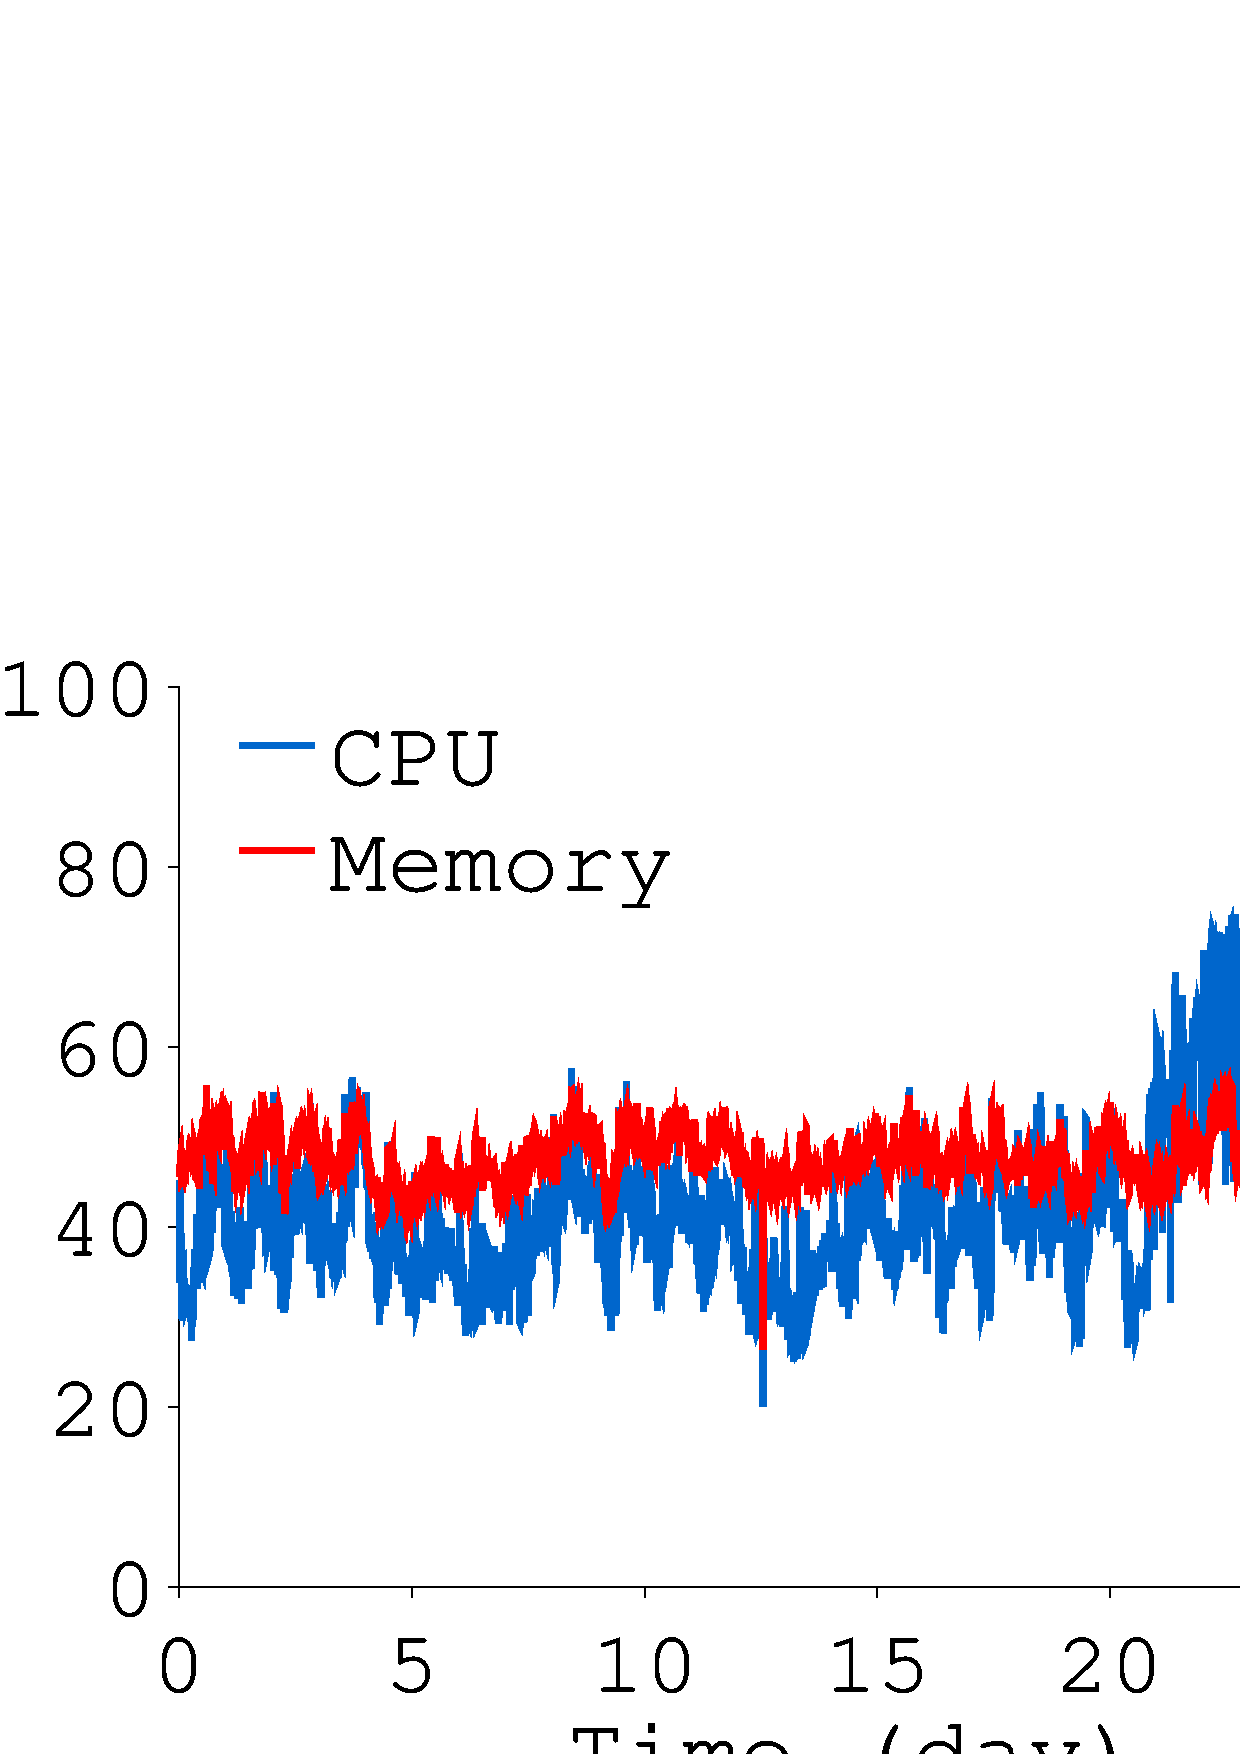
\includegraphics[width=3in]{lego/Figures/g_plot_google_util.pdf}}
    \caption[Google Cluster.]{Google Cluster.}
    \label{fig-googleutil}    
    \end{center}
\end{subfigure}
\begin{subfigure}{3in}
    \begin{center}    
    \centerline{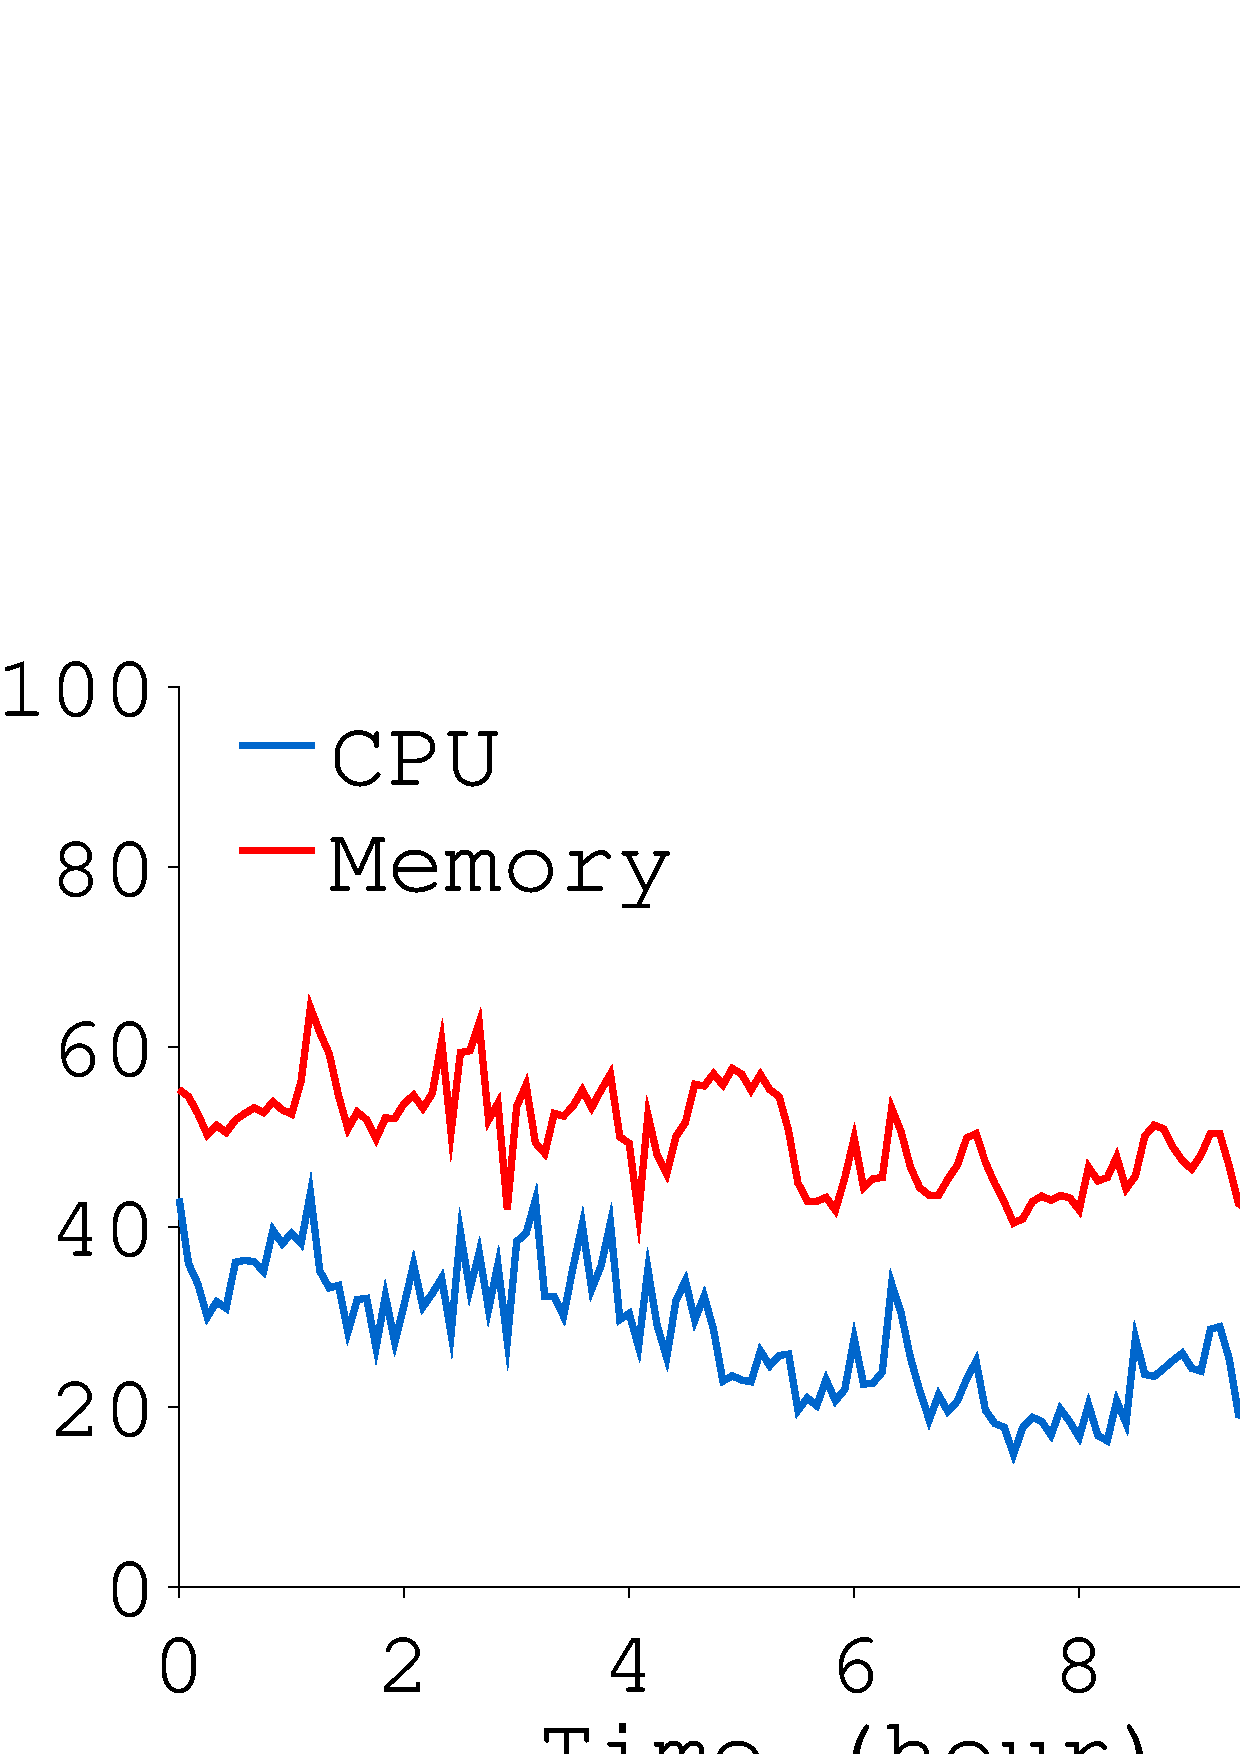
\includegraphics[width=3in]{lego/Figures/g_plot_ali_util.pdf}}    
    \caption[Alibaba Cluster.]{Alibaba Cluster.}
    \label{fig-aliutil}
    \end{center}    
\end{subfigure}
\caption[Data center resource utilization.]{Data center resource utilization.}
\label{fig-resource-anal}
\end{figure}
}
{
\begin{figure*}[t]
\begin{subfigure}{1.7in}
\begin{center}
\centerline{\includegraphics[width=1.7in]{lego/Figures/monolithic-arch.pdf}}
\caption[Monolithic OS.]{OSes Designed for Monolithic Servers.}
\label{fig-monolithic}
\end{center}
\end{subfigure}
\begin{minipage}{0.05in}
\hspace{0.05in}
\end{minipage}
\begin{subfigure}{1.8in}
\begin{center}
\centerline{\includegraphics[width=1.8in]{lego/Figures/multikernel-arch.pdf}}
\caption[Multikernel Architecture.]{Multi-kernel Architecture. \small{P-NIC: programmable NIC.}}
\label{fig-multikernel}
\end{center}
\end{subfigure}
\begin{minipage}{0.05in}
\hspace{0.05in}
\end{minipage}
\begin{subfigure}{2.5in}
\begin{center}
\centerline{\includegraphics[width=2.6in]{lego/Figures/lego-arch.pdf}}
\caption[Splitkernel Architecture.]{Splitkernel Architecture.}
\label{fig-splitkernel}
\end{center}
\end{subfigure}
\caption[Operating System Architecture.]{Operating System Architecture.}
\end{figure*}
}

This section
motivates the hardware resource disaggregation architecture
and discusses the challenges in managing disaggregated hardware.

\subsection{Limitations of Monolithic Servers}
\label{sec:lego:monolimit}
A monolithic server has been the unit of deployment and operation in datacenters for decades.
This long-standing {\em server-centric} architecture has several key limitations.

\noindent{\textit{\uline{Inefficient resource utilization.}}}
With a server being the physical boundary of resource allocation, 
it is difficult to fully utilize all resources in a datacenter~\cite{Barroso-COMPUTER,Quasar-ASPLOS,PowerNap}.
We analyzed two production cluster traces: a 29-day Google one~\cite{GoogleTrace}
and a 12-hour Alibaba one~\cite{AliTrace}.
Figure~\ref{fig-resource-anal} plots the aggregated CPU and memory utilization in the two clusters.
For both clusters, only around half of the CPU and memory are utilized.
Interestingly,
a significant amount of jobs are being evicted at the same time in these traces
(\eg, evicting low-priority jobs to make room for high-priority ones~\cite{Borg}).
One of the main reasons for resource under-utilization in these production clusters is 
the constraint that CPU and memory for a job have to be allocated from 
the same physical machine.

\noindent{\textit{\uline{Poor hardware elasticity.}}}
It is difficult to add, move, remove, or reconfigure hardware components
after they have been installed in a monolithic server~\cite{FB-Wedge100}. %, and
Because of this rigidity, datacenter owners have to plan out server configurations in advance.
However, with today's speed of change in application requirements, such plans have to be adjusted frequently,
and when changes happen, it often comes with waste in existing server hardware.

\noindent{\textit{\uline{Coarse failure domain.}}}
The failure unit of monolithic servers is coarse.
When a hardware component within a server fails, %(\eg, processor, memory chip, RAID controller), 
the whole server is often unusable and applications running on it can all crash.
Previous analysis~\cite{Failure-Disk-FAST07} found that motherboard, memory, CPU, power supply failures account for 
50\% to 82\% of hardware failures in a server.
Unfortunately, monolithic servers cannot continue to operate when any of these devices fail.

\noindent{\textit{\uline{Bad support for heterogeneity.}}}
Driven by application needs, new hardware technologies are finding their ways into modern datacenters~\cite{sigarch-dc}.
Datacenters no longer host only commodity servers with CPU, DRAM, and hard disks. 
They include non-traditional and specialized hardware like GPGPU~\cite{GPU-google,GPU-aws}, 
TPU~\cite{TPU}, 
DPU~\cite{DPU},
FPGA~\cite{Putnam14-FPGA,Amazon-F1}, %,SmartNIC-nsdi18},
non-volatile memory~\cite{Intel3DXpoint}, %,facebook-eurosys18},
and NVMe-based SSDs~\cite{everspin}.
The monolithic server model tightly couples hardware devices with each other and with a motherboard.
As a result, making new hardware devices work with existing servers is a painful and lengthy process~\cite{Putnam14-FPGA}.
%The current practice of making new hardware work is not only slow but also expensive.
Mover, datacenters often need to purchase new servers to host certain hardware.
Other parts of the new servers can go underutilized 
and old servers need to retire to make room for new ones.

\subsection{Hardware Resource Disaggregation}
The server-centric architecture is a bad fit for the fast-changing datacenter hardware, software, and cost needs.
There is an emerging interest in utilizing resources beyond a local machine~\cite{Gao16-OSDI},
such as distributed memory~\cite{Dragojevic14-FaRM,Nelson15-ATC,Aguilera17-SOCC,Novakovic16-SOCC} and network swapping~\cite{GU17-NSDI}. 
These solutions improve resource utilization over traditional systems.
However, they cannot solve all the issues of monolithic servers (\eg, the last three issues in \S\ref{sec:lego:monolimit}), 
since their hardware model is still a monolithic one.
To fully support the growing heterogeneity in hardware and to provide elasticity and flexibility at the hardware level, 
we should {\em break the monolithic server model.}% into flexible resource components.

We envision a {\em hardware resource disaggregation} architecture 
where hardware resources in traditional servers are disseminated into network-attached {\em hardware components}.
Each component has a controller and a network interface,
can operate on its own,
and is an {\em independent, failure-isolated} entity.

The disaggregated approach largely increases the flexibility of a datacenter.
Applications can freely use resources from any hardware component,
which makes resource allocation easy and efficient.
Different types of hardware resources can {\em scale independently}.
It is easy to add, remove, or reconfigure components.
New types of hardware components can easily be deployed in a datacenter ---
by simply enabling the hardware to talk to the network and adding a new network link to connect it.
Finally, hardware resource disaggregation enables fine-grain failure isolation, % because of decomposed hardware resources.
since one component failure will not affect the rest of a cluster.

Three hardware trends are making resource disaggregation feasible in datacenters.
First, network speed has grown by more than an order of magnitude and has become more scalable in the past decade % faster both in bandwidth and latency
with new technologies like Remote Direct Memory Access ({\it RDMA})~\cite{ibverbs} 
and new topologies and switches~\cite{FireBox-FASTKeynote,costa15-r2c2,Costa-WRSC14},
enabling fast accesses of hardware components that are disaggregated across the network.
InfiniBand will soon reach 200Gbps and sub-600 nanosecond speed~\cite{Mellanox-ConnectX6-IB},
being only 2\x\ to 4\x\ slower than main memory bus in bandwidth.
With main memory bus facing a bandwidth wall~\cite{BW-Wall-ISCA09},
future network bandwidth (at line rate) is even projected to exceed local DRAM bandwidth~\cite{CacheCloud-hotcloud18}.

Second, network interfaces are moving closer to hardware components,
with technologies like Intel OmniPath~\cite{OmniPath},
RDMA~\cite{ibverbs},
and NVMe over Fabrics~\cite{NVMe-fabrics-Inteltalk,NVMe-fabrics}.
As a result, hardware devices will be able to access network directly 
without the need to attach any processors. 

Finally, hardware devices are incorporating more processing power~\cite{Ahn15-PIM,Bojnordi12,Mellanox-SmartNIC,Mellanox-SmartNIC2,Agilio-SmartNIC,Junwhan-ISCA17},
allowing application and OS logics to be offloaded to hardware~\cite{Willow,Kaufmann16-ASPLOS}.
On-device processing power will enable system software to manage disaggregated hardware components locally.

With these hardware trends and the limitations of monolithic servers,
we believe that future datacenters will be able to largely benefit from hardware resource disaggregation.
In fact, there have already been several initial hardware proposals in resource disaggregation~\cite{OCP},
including disaggregated memory~\cite{Lim09-disaggregate,Scaleout-numa,Nitu18-EUROSYS}, 
disaggregated flash~\cite{FlashDisaggregation,ReFlex},
%new power state for disaggregated memory~\cite{Nitu18-EUROSYS},
Intel Rack-Scale System~\cite{IntelRackScale}, 
HP ``The Machine''~\cite{HP-TheMachine,HP-MemoryOS}, 
IBM Composable System~\cite{IBM-Composable},
and Berkeley Firebox~\cite{FireBox-FASTKeynote}.

\subsection{OSes for Resource Disaggregation}
Despite various benefits hardware resource disaggregation promises, 
it is still unclear how to manage or utilize disaggregated hardware in a datacenter.
Unfortunately, existing OSes and distributed systems cannot work well with this new architecture.
Single-node OSes like Linux view a server as the unit of management and assume all hardware components are local (Figure~\ref{fig-monolithic}).
A potential approach is to run these OSes on processors
and access memory, storage, and other hardware resources remotely.
Recent disaggregated systems like soNUMA~\cite{Scaleout-numa} take this approach.
However, this approach incurs high network latency and bandwidth consumption with remote device management,
misses the opportunity of exploiting device-local computation power,
and makes processors the single point of failure.

Multi-kernel solutions~\cite{Baumann-SOSP09,Barrelfish-DC,Helios-SOSP,fos-SOCC,Hive-SOSP} (Figure~\ref{fig-multikernel}) 
view different cores, processors, or programmable devices within a server separately 
by running a kernel on each core/device and using message passing to communicate across kernels.
These kernels still run in a single server and all access some common hardware resources in the server like memory and the network interface.
Moreover, they do not manage distributed resources or handle failures in a disaggregated cluster. 

There have been various distributed OS proposals,
most of which date decades back~\cite{Amoeba-Experience,Sprite,MOSIX}. %,V-System,Accent-SOSP,DEMOS-SOSP,Charlotte}.
Most of these distributed OSes manage a set of monolithic servers
instead of hardware components.

Hardware resource disaggregation is fundamentally different from the traditional monolithic server model.
A complete disaggregation of processor, memory, and storage 
means that when managing one of them, there will be no local accesses to the other two.
For example, processors will have no local memory or storage to store user or kernel data.
%Memory and storage components will only have limited processing power. %not have no local memory to serve as cache.
An OS also needs to manage distributed hardware resource and handle hardware component failure.
We summarize the following key challenges in building an OS for resource disaggregation,
some of which have previously been identified~\cite{HP-MemoryOS}.

\begin{itemize}
\item How to deliver good performance when application execution involves the access of network-partitioned disaggregated hardware
and current network is still slower than local buses?

\item How to locally manage individual hardware components with limited hardware resources?

%\item How to communicate across components?

\item How to manage distributed hardware resources?

\item How to handle a component failure without affecting other components or running applications?

\item What abstraction should be exposed to users and how to support existing datacenter applications?

\end{itemize}

Instead of retrofitting existing OSes to confront these challenges,
we take the approach of designing a new OS architecture from the ground up for hardware resource disaggregation.

\section{Distributed Shared Persistent Memory}
\label{sec:dspm}

The datacenter application and hardware trends described in Section~\ref{sec:motivation} 
clearly point to one promising direction of using \nvm\ in datacenter environments --- 
as distributed, shared, persistent memory (\dsnvm).
A \dsnvm\ system manages a distributed set of \nvm{}-equipped machines  
and provides the abstraction of a global virtual address space and a data persistence interface to applications.
This section gives a brief discussion on the \dsnvm\ model.

\subsection{\dsnvm\ Benefits and Usage Scenarios}
\dsnvm\ offers low-latency, shared access to vast amount of durable data in distributed \nvm,
and the reliability and high availability of these data.
Application developers can build in-memory data structures with the global virtual address space 
and decide how to name their data and when to make data persistent.

Applications that fit \dsnvm\ well have two properties:
accessing data with memory instructions and making data durable explicitly.
We call the time when an application makes its data persistent a {\em commit point}.
There are several types of datacenter applications that meet the above two descriptions and can benefit from running on \dsnvm.

First, applications that are built for single-node \nvm\
can be easily ported to \dsnvm\ and scale out to distributed environments.
These applications store persistent data as in-memory data structures 
and already express their commit points explicitly.
Similarly, storage applications that use memory-mapped files also fit \dsnvm\ well,
since they operate on in-memory data and explicitly make them persistent at well-defined commit points (\ie, \msync).
Finally, \dsnvm\ fits shared-memory or DSM-based applications that desire to incorporate durability.
These applications do not yet have durable data commit points,
but we expect that when developers want to make their applications durable, 
they should have the knowledge of when and what data they want make durable.

\subsection{\dsnvm\ Challenges}
\label{sec:challenges}
Building a \dsnvm\ system presents several new challenges.

First, {\em what type of abstraction should \dsnvm\ offer to support both direct memory accesses and data persistence (Section~\ref{sec:abstraction})}?
To perform native memory accesses, application processes should use virtual memory addresses. 
But virtual memory addresses are not a good way to {\em name} persistent data.
\dsnvm\ needs a naming mechanism that applications can easily use to retrieve their in-memory data after reboot or crashes (Section~\ref{sec:naming}).
Allowing direct memory accesses to \dsnvm\ also brings another new problem:
pointers need to be both persistent in \nvm\ and consistent across machines (Section~\ref{sec:addressing}).

Second, {\em how to efficiently organize data in \dsnvm\ to deliver good application performance (Section~\ref{sec:data})?}
To make \dsnvm's interface easy to use and transparent, 
\dsnvm\ should manage the physical \nvm\ space for applications and handle \nvm\ allocation.
\dsnvm\ needs a flexible and efficient data management mechanism to deliver good performance to different types of applications.

Finally, {\em \dsnvm\ needs to ensure both distributed cache coherence and data reliability at the same time} (Section~\ref{sec:xact}).
The former requirement ensures the coherence of multiple cached copies at different machines under concurrent accesses and is usually enforced in a distributed memory layer.
The latter provides data reliability and availability when crashes happen and is implemented in distributed storage systems or distributed databases.
\dsnvm\ needs to incorporate both these two different requirements in one layer in a correct and efficient way.
%Note that PM is attached to main memory bus directly, hence we assume PM share the same CPU cache coherence mechanism with DRAM.
%Hotpot focus on cache coherence among different cached copies across nodes.

\section{\lego\ Design}
\label{sec:lego:design}

Based on the \splitkernel\ architecture,
we built {\em \lego}, the first OS designed for hardware resource disaggregation.
\lego\ is a research prototype that demonstrates the feasibility of the \splitkernel\ design,
but it is not the only way to build a \splitkernel.
\lego' design targets three types of hardware components:
processor, memory, and storage,
and we call them {\em \pcomponent, \mcomponent}, and {\em \scomponent}.

This section first introduces the abstraction \lego\ exposes to users
and then describes the hardware architecture of components \lego\ runs on.
Next, we explain the design of \lego' process, memory, and storage \microos{}s.
Finally, we discuss \lego' global resource management and failure handling mechanisms.

Overall, \lego\ achieves the following design goals:

\begin{itemize}

\item Clean separation of process, memory, and storage functionalities.

\item Monitors run at hardware components and fit device constraints.

\item Comparable performance to monolithic Linux servers.

\item Efficient resource management and memory failure handling, both in space and in performance. % and performance-efficient memory replication scheme.

\item Easy-to-use, backward compatible user interface.

\item Supports common Linux system call interfaces.

\end{itemize}

\subsection{Abstraction and Usage Model}
\lego\ exposes a distributed set of {\em virtual nodes}, or {\em \vnode}, to users.
From users' point of view, a \vnode\ is like a virtual machine. 
Multiple users can run in a \vnode\ and each user can run multiple processes.
Each \vnode\ has a unique ID, a unique virtual IP address, %({\em \vip}),
and its own storage mount point. % ({\em \vmount}).
\lego\ protects and isolates the resources given to each \vnode\ from others.
Internally, one \vnode\ can run on multiple \pcomponent{}s, multiple \mcomponent{}s,
and multiple \scomponent{}s.
At the same time, each hardware component can host resources for more than one \vnode.
The internal execution status is transparent to \lego\ users;
they do not know which physical components their applications run on.

With \splitkernel's design principle of components not being coherent,
\lego\ does not support writable shared memory across processors. %execute application threads that need to have shared write access to common memory.
\lego\ assumes that threads within the same process access shared memory
and threads belonging to different processes do not share writable memory,
and \lego\ makes scheduling decision based on this assumption (\S\ref{sec:lego:proc-scheduling}).
Applications that use shared writable memory across processes (\eg, with MAP\_SHARED)
will need to be adapted to use message passing across processes.
We made this decision because writable shared memory across processes is rare 
(we have not seen a single instance in the datacenter applications we studied),
and supporting it makes both hardware and software more complex 
(in fact, we have implemented this support but later decided not to include it because of its complexity).

One of the initial decisions we made when building \lego\ is to support the Linux system call interface 
and unmodified Linux ABI,
because doing so can greatly ease the adoption of \lego.
Distributed applications that run on Linux can seamlessly run on a \lego\ cluster
by running on a set of \vnode{}s. % and using their virtual IP addresses to communicate.

\subsection{Hardware Architecture}
\label{sec:lego:hardware}
{
\begin{figure}[th]
\begin{center}
\centerline{\includegraphics[width=0.8\textwidth]{lego/Figures/hwarch.pdf}}
\caption[\lego\ \pcomponent\ and \mcomponent\ Architecture.]{\lego\ \pcomponent\ and \mcomponent\ Architecture.}
\label{fig-lego-hw-arch}
\end{center}
\end{figure}
}

\lego\ \pcomponent, \mcomponent, and \scomponent\ are independent devices,
each having their own hardware controller and network interface (for \pcomponent, the hardware controller is the processor itself).
Our current hardware model uses CPU in \pcomponent, 
DRAM in \mcomponent, and SSD or HDD in \scomponent.
We leave exploring other hardware devices for future work.

To demonstrate the feasibility of hardware resource disaggregation,
we propose a \pcomponent{} and an \mcomponent\ architecture designed 
within today's network, processor, and memory performance and hardware constraints
(Figure~\ref{fig-lego-hw-arch}).

\noindent{\textit{\uline{Separating process and memory functionalities.}}}
\lego\ moves all hardware memory functionalities to \mcomponent{}s 
(e.g., page tables, TLBs) and leaves {\em only} caches at the \pcomponent{} side. 
With a clean separation of process and memory hardware units, 
the allocation and management of memory can be completely transparent to \pcomponent{}s.
Each \mcomponent{} can choose its own memory allocation technique
and virtual to physical memory address mappings (\eg, segmentation). 

\noindent{\textit{\uline{Processor virtual caches.}}}
After moving all memory functionalities to \mcomponent{}s,  
\pcomponent{}s will only see virtual addresses and have to use virtual memory addresses to access its caches. 
Because of this, \lego\ organizes all levels of \pcomponent{} caches as {\em virtual caches}~\cite{Goodman-ASPLOS87,Wang-ISCA89},
\ie, virtually-indexed and virtually-tagged caches.

A virtual cache has two potential problems, commonly known as synonyms and homonyms~\cite{CacheMemory82}.
Synonyms happens when a physical address maps to multiple virtual addresses (and thus multiple virtual cache lines) 
as a result of memory sharing across processes,
and the update of one virtual cache line will not reflect to other lines that share the data.
Since \lego\ does not allow writable inter-process memory sharing,
it will not have the synonym problem.
The homonym problem happens when two address spaces use the same virtual address for their own different data.
Similar to previous solutions~\cite{OVC}, we solve homonyms by storing an address space ID (ASID) with each cache line,
and differentiate a virtual address in different address spaces using ASIDs.

\noindent{\textit{\uline{Separating memory for performance and for capacity.}}}
Previous studies~\cite{Gao16-OSDI,GU17-NSDI} and our own show that today's network speed 
cannot meet application performance requirements if all memory accesses are across the network. 
Fortunately, many modern datacenter applications exhibit strong memory access temporal locality.
For example, we found 90\% of memory accesses in PowerGraph~\cite{Gonzalez12-OSDI} go to just 0.06\% of total memory
and 95\% go to 3.1\% of memory
(22\% and 36\% for TensorFlow~\cite{TensorFlow} respectively,
5.1\% and 6.6\% for Phoenix~\cite{Ranger07-HPCA}).
%PG 90% 0.0063G 95% 0.301G 100% 9.68G
%TF 90% 0.608G 95% 0.968G 100% 2.7G

With good memory-access locality, we propose to %separate hardware memory into two categories and organize them differently:
leave a small amount of memory (\eg, 4\GB) at each \pcomponent{}
and move most memory across the network (\eg, few TBs per \mcomponent{}).
\pcomponent{}s' local memory can be regular DRAM 
or the on-die HBM~\cite{HBM-JEDEC,Knights-Landing},
and \mcomponent{}s use DRAM or NVM.

Different from previous proposals~\cite{Lim09-disaggregate}, 
we propose to organize \pcomponent{}s' DRAM/HBM as cache rather than main memory
for a clean separation of process and memory functionalities.
We place this cache under the current processor Last-Level Cache (LLC)
and call it an extended cache, or {\em \excache}.
\excache\ serves as another layer in the memory hierarchy between LLC and memory across the network.
With this design, \excache\ can serve hot memory accesses fast, while \mcomponent{}s can provide the capacity applications desire. 

\excache\ is a virtual, inclusive cache,
and we use a combination of hardware and software to manage \excache.
Each \excache\ line has a (virtual-address) tag and two access permission bits (one for read/write and one for valid).
These bits are set by software when a line is inserted to \excache\ and checked by hardware at access time.
For best hit performance, the hit path of \excache\ is handled purely by hardware
--- the hardware cache controller maps a virtual address to an \excache\ set, 
fetches and compares tags in the set, and on a hit, fetches the hit \excache\ line.
Handling misses of \excache\ is more complex than with traditional CPU caches, 
and thus we use \lego\ to handle the miss path of \excache\ (see \S\ref{sec:lego:excachemgmt}).

Finally, we use a small amount of DRAM/HBM at \pcomponent{} for \lego' own kernel data usages,
accessed directly with physical memory addresses and managed by \lego. 
\lego\ ensures that all its own data fits in this space to avoid going to \mcomponent{}s.

With our design, \pcomponent{}s do not need any address mappings:
\lego\ accesses all \pcomponent{}-side DRAM/HBM using physical memory addresses
and does simple calculations to locate the \excache\ set for a memory access.
Another benefit of not handling address mapping at \pcomponent{}s and moving TLBs to \mcomponent{}s 
is that \pcomponent{}s do not need to access TLB or suffer from TLB misses,
potentially making \pcomponent{} cache accesses faster~\cite{Kaxiras-ISCA13}.
%We use software~\cite{softvm-HPCA97,Tsai-ISCA17} (\lego) to manage \excache\ and the kernel physical memory,
%although they can all be implemented in hardware too.

\subsection{Process Management}
The \lego\ {\em process \microos{}} runs in the kernel space of a \pcomponent\
and manages the \pcomponent's CPU cores and \excache. 
\pcomponent{}s run user programs in the user space.

\subsubsection{Process Management and Scheduling}
\label{sec:lego:proc-scheduling}
At every \pcomponent, \lego\ uses a simple local thread scheduling model 
that targets datacenter applications 
(we will discuss global scheduling in \S~\ref{sec:lego:grm}).
\lego\ dedicates a small amount of cores for kernel background threads 
(currently two to four)
and uses the rest of the cores for application threads.
When a new process starts, \lego\ uses a global policy to choose a \pcomponent{} for it (\S~\ref{sec:lego:grm}).
Afterwards, \lego\ schedules new threads the process spawns on the same \pcomponent{} 
by choosing the cores that host fewest threads.
After assigning a thread to a core, 
we let it run to the end with no scheduling or kernel preemption under common scenarios.
For example, we do not use any network interrupts 
and let threads busy wait on the completion of outstanding network requests, 
since a network request in \lego\ is fast 
(\eg, fetching an \excache\ line from an \mcomponent\ takes around 6.5\mus).
\lego\ improves the overall processor utilization in a disaggregated cluster,
since it can freely schedule processes on any \pcomponent{}s without considering memory allocation.
Thus, we do not push for perfect core utilization when scheduling individual threads
and instead aim to minimize scheduling and context switch performance overheads.
Only when a \pcomponent{} has to schedule 
more threads than its cores will
\lego\ start preempting threads on a core.

\subsubsection{\excache\ Management}
\label{sec:lego:excachemgmt}
\lego\ process \microos\ configures and manages \excache.
During the \pcomponent{}'s boot time, \lego\ configures the set associativity of \excache\
and its cache replacement policy.
While \excache\ hit is handled completely in hardware, 
\lego\ handles misses in software.
When an \excache\ miss happens, 
the process \microos\ fetches the corresponding line from an \mcomponent\ and inserts it to \excache.
If the \excache\ set is full, the process \microos\ first evicts a line in the set.
It throws away the evicted line if it is clean
and writes it back to an \mcomponent{} if it is dirty.
\lego\ currently supports two eviction policies: FIFO and LRU.
For each \excache\ set, \lego\ maintains a FIFO queue (or an approximate LRU list)
and chooses \excache\ lines to evict based on the corresponding policy (see \S\ref{sec:lego:procimpl} for details).

\subsubsection{Supporting Linux Syscall Interface}
One of our early decisions is to support Linux ABIs for backward compatibility
and easy adoption of \lego.
A challenge in supporting the Linux system call interface is that 
many Linux syscalls are associated with {\em states},
information about different Linux subsystems that is stored with each process 
and can be accessed by user programs across syscalls.
For example, Linux records the states of a running process' open files, socket connections, and several other entities,
and it associates these states with file descriptors ({\em fd}s) that are exposed to users.
In contrast, \lego\ aims at the clean separation of OS functionalities.
With \lego' stateless design principle, each component only stores information about its own resource
and each request across components contains all the information that the destination component needs to handle the request.
To solve this discrepancy between the Linux syscall interface and \lego' design, 
we add a layer on top of \lego' core process \microos\ at each \pcomponent\ to store Linux states
and translate these states and the Linux syscall interface to \lego' internal interface.

\subsection{Memory Management}

We use \mcomponent{}s for three types of data:
anonymous memory (\ie, heaps, stacks), 
memory-mapped files, and storage buffer caches.
The \lego\ {\em memory \microos{}}
manages both the virtual and physical memory address spaces,
their allocation, deallocation, and memory address mappings.
It also performs the actual memory read and write.
No user processes run on \mcomponent{}s 
and they run completely in the kernel mode
(same is true for \scomponent{}s). 

\lego\ lets a process address space span multiple \mcomponent{}s
to achieve efficient memory space utilization and high parallelism.
Each application process uses one or more \mcomponent{}s to host its data
and a {\em home \mcomponent},
an \mcomponent\ that initially loads the process, 
accepts and oversees all system calls related to virtual memory space management
(\eg, \brk, \mmap, \munmap, and \mremap).
\lego\ uses a global memory resource manager ({\em \gmm}) to assign a home \mcomponent{} to each new process at its creation time.
A home \mcomponent\ can also host process data.

\subsubsection{Memory Space Management}
\noindent{\textit{\uline{Virtual memory space management.}}}
We propose a two-level approach to manage distributed virtual memory spaces,
where the home \mcomponent\ of a process makes coarse-grained, high-level virtual memory allocation decisions
and other \mcomponent{}s perform fine-grained virtual memory allocation.
This approach minimizes network communication during both normal memory accesses and virtual memory operations,
while ensuring good load balancing and memory utilization.
Figure~\ref{fig-dist-vma} demonstrates the data structures used. % in virtual memory space management.

At the higher level, we split each virtual memory address space into coarse-grained, fix-sized {\em virtual regions},
or {\em \vregion{}s} (\eg, of 1\GB).
Each \vregion\ that contains allocated virtual memory addresses (an active \vregion) is {\em owned} by an \mcomponent{}.
The owner of a \vregion\ handles all memory accesses and virtual memory requests within the \vregion.

{
\begin{figure}[th]
\begin{minipage}{\figWidth}
\begin{center}
\centerline{\includegraphics[width=2.8in]{Figures/dist-vma.pdf}}
%\vspace{-0.1in}
\mycaption{fig-dist-vma}{Distributed Memory Management.}
{
}
\end{center}
\end{minipage}
\vspace{-0.15in}
\end{figure}
}

The lower level stores user process virtual memory area ({\em vma}) information,
such as virtual address ranges and permissions, in {\em vma trees}.
The owner of an active \vregion\ stores a vma tree for the \vregion,
with each node in the tree being one vma.
A user-perceived virtual memory range can split across multiple \mcomponent{}s,
but only one \mcomponent{} owns a \vregion.

\vregion\ owners perform the actual virtual memory allocation and vma tree set up.
A home \mcomponent{} can also be the owner of \vregion{}s,
but the home \mcomponent{} does not maintain any information about memory that belongs to \vregion{}s owned by other \mcomponent{}s.
It only keeps the information of which \mcomponent{} owns a \vregion\ (in a {\em \vregion\ array})
and how much free virtual memory space is left in each \vregion.
These metadata can be easily reconstructed if a home \mcomponent{} fails.

When an application process wants to allocate a virtual memory space,
the \pcomponent{} forwards the allocation request 
to its home \mcomponent{} (\circled{1} in Figure~\ref{fig-dist-vma}).
The home \mcomponent{} uses its stored information of available virtual memory space in \vregion{}s
to find one or more \vregion{}s that best fit the requested amount of virtual memory space.
If no active \vregion\ can fit the allocation request, the home \mcomponent{} makes a new \vregion\ active and 
contacts the \gmm\ (\circled{2} and \circled{3}) to find a candidate \mcomponent{} to own the new \vregion.
\gmm\ makes this decision based on available physical memory space and access load on different \mcomponent{}s (\S~\ref{sec:lego:grm}).
If the candidate \mcomponent\ is not the home \mcomponent{}, the home \mcomponent{} next forwards the request to that \mcomponent\ (\circled{4}),
which then performs local virtual memory area allocation and sets up the proper vma tree. 
Afterwards, the \pcomponent{} directly sends memory access requests to the owner of the \vregion\ where the memory access falls into
(\eg, \circled{a} and \circled{c} in Figure~\ref{fig-dist-vma}).


\lego' mechanism of distributed virtual memory management is efficient and it cleanly separates memory operations from \pcomponent{}s.
\pcomponent{}s hand over all memory-related system call requests to \mcomponent{}s
and only cache a copy of the \vregion\ array for fast memory accesses.
To fill a cache miss or to flush a dirty cache line, 
a \pcomponent{} looks up the cached \vregion\ array to find its owner \mcomponent{} and sends the request to it.

\noindent{\textit{\uline{Physical memory space management.}}}
Each \mcomponent\ manages the physical memory allocation for data that falls into the
\vregion\ that it owns.
Each \mcomponent{} can choose their own way of physical memory allocation
and own mechanism of virtual-to-physical memory address mapping.


\subsubsection{Optimization on Memory Accesses}
\label{sec:lego:zerofill}
With our strawman memory management design, 
all \excache\ misses will go to \mcomponent{}s.
We soon found that a large performance overhead in running real applications 
is caused by filling empty \excache, \ie, {\em cold misses}.
To reduce the performance overhead of cold misses, we propose a technique 
to avoid accessing \mcomponent\ on first memory accesses.

The basic idea is simple: since the initial content of anonymous memory 
(non-file-backed memory) is zero, %undefined and can be any data, 
\lego\ can directly allocate a cache line with empty content
in \excache\ for the first access to 
anonymous memory instead of going to \mcomponent\
(we call such cache lines {\em p-local lines}).
When an application creates a new anonymous memory region, the process \microos\ records its address range and permission.
The application's first access to this region will be an \excache\ miss and it will trap to \lego.
\lego\ process \microos\ then allocates an \excache\ line, fills it with zeros, 
and sets its R/W bit according to the recorded memory region's permission.
Before this p-local line is evicted, it only lives in the \excache.
No \mcomponent{}s are aware of it or will allocate physical memory or a virtual-to-physical memory mapping for it.
When a p-local cache line becomes dirty and needs to be flushed, 
the process \microos\ sends it to its owner \mcomponent, which then
allocates physical memory space and establishes a virtual-to-physical memory mapping.
Essentially, \lego\ {\em delays physical memory allocation until write time}.
Notice that it is safe to only maintain p-local lines at a \pcomponent{} \excache\ 
without any other \pcomponent{}s knowing them, 
since \pcomponent{}s in \lego\ do not share any memory
and other \pcomponent{}s will not access this data.

\subsection{Storage Management}
\lego\ supports a hierarchical file interface that is backward compatible with POSIX 
through its \vnode\ abstraction. 
Users can store their directories and files under their \vnode{}s' mount points
and perform normal read, write, and other accesses to them.

\lego\ implements core storage functionalities at \scomponent{}s.
To cleanly separate storage functionalities, \lego\ uses a stateless storage server design, 
where each I/O request to the storage server contains all the information needed to 
fulfill this request, \eg, full path name, absolute file offset,
similar to the server design in NFS v2~\cite{Sandberg-NFS-85}.

While \lego\ supports a hierarchical file use interface,
internally, \lego\ storage \microos\ treats (full) directory and file paths just as unique names of a file
and place all files of a \vnode\ under one internal directory at the \scomponent{}.
To locate a file, \lego\ storage \microos\ maintains a simple hash table with the full paths of files (and directories) as keys.
From our observation, most datacenter applications only have a few hundred files or less.
Thus, a simple hash table for a whole \vnode\ is sufficient to achieve good lookup performance.
Using a non-hierarchical file system implementation largely reduces the complexity of \lego' file system,
making it possible for a storage \microos\ to fit in storage devices controllers that have limited processing power~\cite{Willow}.

\lego\ places the storage buffer cache at \mcomponent{}s
rather than at \scomponent{}s, because \scomponent{}s can only host a limited amount of internal memory.
\lego\ memory \microos\ manages the storage buffer cache by simply performing insertion, lookup, and deletion of buffer cache entries.
For simplicity and to avoid coherence traffic, we currently place the buffer cache of one file
under one \mcomponent{}.
When receiving a file read system call, the \lego\ process \microos\ first uses its extended Linux state layer to 
look up the full path name, then passes it with the requested offset and size to the \mcomponent\ that holds the file's buffer cache.
This \mcomponent\ will look up the buffer cache and returns the data to \pcomponent\ on a hit.
On a miss, \mcomponent\ will forward the request to the \scomponent\ that stores the file, 
which will fetch the data from storage device and return it to the \mcomponent.
The \mcomponent\ will then insert it into the buffer cache and returns it to the \pcomponent.
Write and fsync requests work in a similar fashion.

\subsection{Global Resource Management}
\label{sec:lego:grm}
\lego\ uses a two-level resource management mechanism.
At the higher level, \lego\ uses three global resource managers for process, memory, and storage resources, 
{\em \gpm, \gmm}, and {\em \gsm}.
These global managers perform coarse-grained global resource allocation and load balancing,
and they can run on one normal Linux machine.
Global managers only maintain approximate resource usage and load information.
They update their information either when they make allocation decisions 
or by periodically asking \microos{}s in the cluster.
At the lower level, each \microos\ can employ its own policies and mechanisms to manage its local resources.

For example, process \microos{}s allocate new threads locally 
and only ask \gpm\ when they need to create a new process.
\gpm\ chooses the \pcomponent{} that has the least amount of threads based on its maintained approximate information.
Memory \microos{}s allocate virtual and physical memory space on their own.
Only home \mcomponent{} asks \gmm\ when it needs to allocate a new \vregion.
\gmm\ maintains approximate physical memory space usages and memory access load by periodically asking \mcomponent{}s
and chooses the memory with least load among all the ones that have at least \vregion\ size of free physical memory.

\lego\ decouples the allocation of different resources and 
can freely allocate each type of resource from a pool of components.
Doing so largely improves resource packing compared to a monolithic server cluster
that packs all type of resources a job requires within one physical machine.
Also note that \lego\ allocates hardware resources only {\em on demand}, 
\ie, when applications actually create threads or access physical memory.
This on-demand allocation strategy further improves \lego' resource packing efficiency
and allows more aggressive over-subscription in a cluster.

\subsection{Reliability and Failure Handling}
\label{sec:lego:failure}
After disaggregation, \pcomponent{}s, \mcomponent{}s, and \scomponent{}s can all fail independently.
Our goal is to build a reliable disaggregated cluster that has the same or lower application failure rate
than a monolithic cluster.
As a first (and important) step towards achieving this goal, %building a reliable disaggregated cluster,
we focus on providing memory reliability by handling \mcomponent\ failure in the current version of \lego\ because of three observations.
First, when distributing an application's memory to multiple \mcomponent{}s, 
the probability of memory failure increases and not handling \mcomponent\ failure will cause applications to fail more often 
on a disaggregated cluster than on monolithic servers.
Second, since most modern datacenter applications
already provide reliability to their distributed storage data %(usually through some form of redundancy)
and the current version of \lego\ does not split a file across \scomponent,
we leave providing storage reliability to applications.
Finally, since \lego\ does not split a process across \pcomponent{}s,
the chance of a running application process being affected by the failure of a \pcomponent\ is similar to 
one affected by the failure of a processor in a monolithic server.
Thus, we currently do not deal with \pcomponent\ failure and leave it for future work.

A naive approach to handle memory failure is to perform a full replication of memory content over two or more \mcomponent{}s.
This method would require at least 2\x\ memory space,
making the monetary and energy cost of providing reliability prohibitively high (the same reason why RAMCloud~\cite{Ongaro11-RamCloud} does not replicate in memory).
Instead, we propose a space- and performance-efficient approach to provide in-memory data reliability in a best-effort way.
Further, since losing in-memory data will not affect user persistent data,
we propose to provide memory reliability in a best-effort manner.

We use one primary \mcomponent, one secondary \mcomponent, and a backup file in \scomponent\ for each vma.
A \mcomponent{} can serve as the primary for some vma and the secondary for others.
The primary stores all memory data and metadata.
\lego\ maintains a small append-only log at the secondary \mcomponent{}
and also replicates the vma tree there.
When \pcomponent{} flushes a dirty \excache\ line, 
\lego\ sends the data to both primary and secondary in parallel (step \circled{a} and \circled{b} in Figure~\ref{fig-dist-vma})
and waits for both to reply (\circled{c} and \circled{d}).
In the background, the secondary \mcomponent\ flushes the backup log to a \scomponent{},
which writes it to an append-only file.

If the flushing of a backup log to \scomponent\ is slow and the log is full, 
we will skip replicating application memory.
If the primary fails during this time, \lego\ simply reports an error to application.
Otherwise when a primary \mcomponent\ fails, we can recover memory content 
by replaying the backup logs on \scomponent\ and in the secondary \mcomponent.
When a secondary \mcomponent\ fails, we do not reconstruct anything 
and start replicating to a new backup log on another \mcomponent{}.


\section{Data Management and Access}
\label{sec:data}

This section presents how \hotpot\ manages user data in \dsnvm. 
We postpone the discussion of data durability and reliability to Section~\ref{sec:xact}.

\subsection{\nvm\ Page Morphable States}
One of \hotpot's design philosophies is to use one layer for both memory and storage 
and to integrate distributed memory caching and data replication.
To achieve this goal, we propose to impose {\em morphable} states on \nvm\ pages,
where the same \nvm\ page in \hotpot\ can be used both as a local memory cached copy to improve performance
and as a redundant data page to improve data reliability and availability.

We differentiate three states of a \nvm\ page:
active and dirty, active and clean, and inactive and clean,
and we call these three states {\em \dirty}, {\em \committed}, and {\em \redundant} respectively.
A page being clean means that it has not been updated since the last commit point;
committing a dirty page moves it to the clean state.
A page being active means that it is currently being accessed by an application,
while an \redundant\ page is a page which the application process has not mapped or accessed.
Several \hotpot\ tasks can change page states,
including page read, page write, data commit, data replication, page migration, and page eviction.
We will discuss how page states change throughout the rest of this section.
Figure~\ref{fig-data-eg} illustrates two operations that cause \hotpot\ data state changes.

\subsection{Data Organization}
\hotpot\ aims to support large-scale, data-intensive applications
on a fairly large number of nodes. %(\eg, at least a few racks)
Thus, it is important to minimize \hotpot's performance and scalability bottlenecks.
In order to enable flexible load balancing and resource management,
\hotpot\ splits the virtual address range of each dataset 
into {\em chunks} of a configurable size (\eg, 4\MB).
\nvm\ pages in a chunk do not need to be physically consecutive
and not all pages in a chunk need to exist on a node.

Each chunk in \hotpot\ is owned by an {\em owner node (\on)},
similar to the ``home'' node in home-based DSM systems~\cite{HLRC}.
%and to the primary node of distributed storage systems,
An \on\ maintains all the data and metadata of the chunk it owns.
%and serves requests from other nodes.
Other nodes, called {\em data node} or {\em \dn}, always fetch data from the \on\
when they initially access the data.
A single \hotpot\ node can simultaneously be the \on\ for some data chunks and the \dn\ for other chunks.
When the application creates a dataset, 
\hotpot\ \cd\ performs an initial assignment of \on{}s to chunks of the dataset.

Two properties separate \hotpot\ \on{}s from traditional home nodes.
First, %besides serving read data,
\hotpot\ \on\ is responsible for the reliability and crash consistency of the pages it owns,
besides serving read data and ensure the coherence of cached copies.
Second, \hotpot\ does not fix which node owns a chunk
and the location of \on\ adapts to application workload behavior dynamically.
Such flexibility is important for load balancing and application performance (see Section~\ref{sec:migration}).

\subsection{Data Reads and Writes}
\label{sec:readwrite}

\hotpot\ minimizes software overhead to improve application performance.
It is invoked only when a page fault occurs or when 
applications execute data persistence operations (see Section~\ref{sec:xact} for details of data persistence operations).

{
\begin{figure}[th]
\centering
\begin{center}
\centerline{\includegraphics[width=\columnwidth]{Figures/data-eg.pdf}}
\end{center}
\vspace{-0.2in}
\mycaption{fig-data-eg}{Data State Change Example.}
{
White, black, and striped blocks represent \committed, \redundant, and \dirty\ states.
Before commit, Node 2 and Node 3 both have cached copies of 
data page $B$. Node 2 has written to $B$ and created a \dirty\ page, $B1$.
During commit, Node 2 pushes the content $B1$ to its \on, Node 1.
Node 1 updates its \committed\ copy to $B1$ and also sends this update to Node 3.
Figure (c) shows the state after migrating the \on\ of chunk 1 from Node 1 to Node 3. 
%page $A$ on Node 3 is \redundant.
After migration, Node 3 has all the pages of the chunk and all of them are in \committed\ states.
}
\vspace{-0.1in}
\end{figure}
}

When a page fault happens because of read, 
it means that there is no valid local page.
\hotpot\ first checks if there is any local \redundant\ page.
If so, it will move this page to the \committed\ state and establish a page table entry (PTE) for it.
Otherwise, there is no available local data and 
\hotpot\ will fetch it from the remote \on.
\hotpot\ writes the received data to a newly-allocated local physical \nvm\ page.
Afterwards, applications will use memory instructions to access this local page directly.


Writing to a \committed\ page also causes a page fault in \hotpot. 
This is because a \committed\ page can contribute towards user-specified degree of replication as one data replica,
and \hotpot\ needs to protect this committed version from being modified.
Thus, \hotpot\ write protects all \committed\ pages.
When these pages are written to (and generating a write page fault), 
\hotpot\ creates a local Copy-On-Write (COW) page
and marks the new page as dirty while leaving
the original page in \committed\ state.
\hotpot\ does not write protect this COW page, since it is already in the dirty state.

Following \hotpot's design philosophy to exploit hints from our targeted data-intensive applications,
we avoid propagating updates to cached copies at other nodes on each write and only do so at each application commit point.
Thus, all writes in \hotpot\ is local and only writing to a \committed\ page will generate a page fault.

Not updating remote cached copies on each write also has the benefit of reducing write amplification in \nvm.
In general, other software mechanisms and policies such as wear-aware \nvm\ allocation and reclamation 
and hardware techniques like Start-Gap~\cite{start-gap-micro09}
can further reduce \nvm\ wear.
We do not focus on \nvm\ wear in this paper and leave such optimizations for future work.

\subsection{\nvm\ Page Allocation and Eviction}
\label{sec:eviction}
Each \hotpot\ node manages its own physical \nvm\ space and performs \nvm\ page allocation and eviction.
Since physical pages do not need to be consecutive,
we use a simple and efficient allocation mechanism by maintaining a free page list
and allocating one page at a time.

\hotpot\ uses an approximate-LRU replacement algorithm that is similar to Linux's page replacement mechanism.
Different from Linux,
\hotpot\ distinguishes pages of different states.
\hotpot\ never evicts a \dirty\ page
and always tries to evict \redundant\ pages before evicting \committed\ pages.
We choose to first evict \redundant\ pages, 
because these are the pages that have not been accessed by applications
and less likely to be accessed in the future than \committed\ pages. %if a node accesses an \redundant\ page, it will become an \committed\ page.

Since both \redundant\ and \committed\ pages can serve as a redundant copy
for data reliability, \hotpot\ cannot simply throw them away during eviction.
The evicting node of a page will contact its \on{}, 
which will check the current degree of replication of the candidate pages 
and prioritize the eviction of pages that already have enough replicas. 
For pages that will drop below the user-defined replication degree after the eviction, 
the \on\ will make a new \redundant\ page at another node. %, if the eviction violates user-specified reliability requirements.

\subsection{Chunk \on\ Migration}
\label{sec:migration}
An \on{} serves both page read and data commit requests that belong to the chunks it owns.
Thus, the location of \on\ is important to \hotpot's performance.
Ideally, the node that performs the most reads and commits of data in a chunk 
should be its \on\ to avoid network communication.

By default, \hotpot\ initially spreads out a dataset's chunks to all \hotpot\ nodes in a round robin fashion
(other static placement policies can easily replace round robin).
Static placement alone cannot achieve optimal run-time performance.
\hotpot\ remedies this limitation by performing online chunk migration,
where one \on\ and one \dn\ of a chunk can switch their identities
and become the new \dn\ and new \on\ of the chunk.

\hotpot\ utilizes application behavior in recent history 
to decide how to migrate \on{}s.
Each \on\ records the number of page read requests
and the amount of committing data it receives in the most recent time window.

\on{}s make their migration decisions with a simple greedy algorithm based on the combination of two criteria:
maximizing the {\em benefit} while not exceeding a configurable {\em cost} of migration.
The benefit is the potential reduction in network traffic during remote data reads and commits.
The node that performs most data communication to the \on\ in recent history
is likely to benefit the most from being the new \on,
since after migration these operations will become local.
We model the cost of migration by the amount of data needed to copy to a node so that it has all the chunk data to become \on.

Once \hotpot\ has made a decision, it performs the actual chunk migration using 
a similar method as process and VM migration~\cite{OsmanEtAl02-Zap,Douglis87-Migration,Clark05-XenMigrate}
by temporary stopping commits to the chunk under migration
and resume them at the new \on\ after migration.

\if 0
    Once decided, a new ON node will be chosen. And the old ON will start to migrate pages to the
    the ON. During migration, the old ON is still the only valid ON in system. And, the old ON
    will keep serving page-fetch, but xact will be rejected.

    Once all pages are migrated from old ON to new ON, the old ON will 1) Tell CD that this region
    is migrated, hence CD can change its metadata. 2) Broadcast to nodes that currently have this
    region, that this region is migrated to new ON.
\fi

\if 0
\subsubsection{Replica Selection}
Apart from \on\ locations, the locations of data replicas can also affect application performance.
When a node has an \redundant\ page it can directly access it and avoid a remote page read. 
Thus, placing a data replica at a node that is likely to access the data in the future
can potentially improve performance.

\hotpot\ \on\ decides where to place an \redundant\ page during transaction commit with two criteria. 
%Currently, we use two criteria in selecting the location of a replica.
%replication gives us a chance to re-balance workloads
%happened in two occasions:
%when committing a transaction 
%and when evicting a \redundant\ page.
First, we use spatial locality to estimate the likelihood a node is going to access an \redundant\ page 
by the number of pages this node has read in the chunk that contains the \redundant\ page.
The second consideration is to prevent thrashing.
When a node runs out of space, it will first evict \redundant\ pages (Section~\ref{sec:eviction})
and assigning \redundant\ pages to such nodes will cause thrashing.
Thus, \hotpot\ compares the total \nvm\ free space of a node and avoids assigning 
\redundant\ pages to nodes with space pressure.
\fi

\section{Data Durability, Consistency, and Reliability}
\label{sec:xact}

Being distributed shared memory and distributed storage at the same time,
\dsnvm\ should ensure both correct shared memory accesses to \nvm\
and the persistence and reliability of in-\nvm\ data. 
\hotpot\ provides three guarantees: coherence among cached copies of in-\nvm\ data,
recovery from various types of failures into a consistent state,
and user data reliability and availability under concurrent failures.
Although each of these three properties have been explored before,
as far as we know, \hotpot\ is the first system that integrates all of them in one layer.
\hotpot\ also has the unique requirement of low software overhead to retain the performance benefit of \nvm.

\begin{itemize}[leftmargin=*]
\item{\em Cache coherence.} 
In \hotpot, application processes on different nodes cache remote data in their local \nvm\ for fast accesses.
\hotpot\ provides two consistency levels across cached copies: 
{\em \ra}, multiple readers and single writer ({\em MRSW}) 
and {\em \rb}, multiple readers and multiple writers ({\em MRMW}).
MRMW allows multiple nodes to concurrently write and commit their local cached copies.
With \mrmw, there can be multiple versions of dirty data in the system (but still one committed version),
while \mrsw\ guarantees only one dirty version at any time.
An application can use different modes for different datasets,
but only one mode with the same dataset.
This design allows flexibility at the dataset granularity while guaranteeing correctness.
 
\item{\em Crash consistency.} 
Data storage applications usually have well-defined {\em consistent} states and need to move from 
one consistent state to another atomically.
When a crash happens, 
user data should be recovered to a consistent state ({\ie, \em crash consistency}). 
\hotpot\ guarantees crash consistency both within a single node ({\em \rcs}) and across distributed nodes ({\em \rcm}).
Note that crash consistency is different and orthogonal to cache
coherence in \ra\ and \rb. 

\item{\em Reliability and availability.} 
To ensure that user persistent data can sustain $N-1$ concurrent node failures, 
where $N$ is a user defined value, \hotpot\ guarantees that {\em \re}, once data has 
been committed, there are always $N$ copies of clean, committed data.

\end{itemize}

This section first discusses how \hotpot\ ensures crash consistency within a single node,
then presents the \mrmw\ and \mrsw\ modes and their atomic commit protocols, %and the optional group fetch protocol.
and ends with the discussion of \hotpot's recovery mechanisms under different crash scenarios.

\subsection{Single-Node Persistence and Consistency}
\label{sec:singleconsistency}

Before ensuring user data's global reliability and consistency in \dsnvm,
\hotpot\ first needs to make sure that data on a single node can properly sustain power crashes (\rcs)~\cite{Memory-Persistency}.
\hotpot\ makes data persistent with the standard Intel persistent memory instructions~\cite{Delegated-persist},
\ie, \clflush, \mfence\ (note that we do not include the deprecated \pcommit\ instruction~\cite{Deprecating-PCOMMIT}).

After a node crashes, if its \nvm\ is still accessible, \hotpot\ will use the \nvm\ content to recover;
otherwise, \hotpot\ will use other nodes to reconstruct data on a new node (Section~\ref{sec:recovery}).
For the former case, \hotpot\ needs to guarantee that user data in \dsnvm\ is in a consistent state after crash.
\hotpot\ also needs to ensure that its own metadata is persistent and is consistent with user data.

\hotpot\ maintains metadata on a local node to find user data and record their morphable states (\ie, \committed, \dirty, or \redundant).
Since these metadata are only used within a single node, \hotpot\ does not need to replicate them on other nodes.
\hotpot\ makes these metadata persistent at known locations in \nvm\ ---
a pre-allocated beginning area of \nvm.
\hotpot\ also uses metadata to record online state of the system (\eg, \on\ maintains a list of active \dn{}s that have a cached copy of data).
These metadata can be reconstructed by re-examining system states after recovery.
Thus, \hotpot\ does not make these metadata persistent.

{
\begin{figure}[t]
\begin{center}
\centerline{\includegraphics[width=\textwidth]{hotpot/Figures/commit.pdf}}
\caption[\mrmw\ Commit Example.]
{
\mrmw\ Commit Example.
Solid arrows represent data communication.
Dashed arrows represent metadata communication.
Node 1 (\xn) commit data to \on{}s at Node 2 and 3 with replication degree four.
Black shapes represent old committed states before the update
and white shapes represent new states.
}
\label{fig-mrmw}
\end{center}
\end{figure}
}

Similar to traditional file systems and databases, 
it is important to enforce {\em ordering} of metadata and data persistence
in order to recover to a consistent state.
For single-node non-commit operations (we defer the discussion of commit operations to Sections \ref{sec:mrmw} and \ref{sec:mrsw}), 
\hotpot\ uses a simple shadow-paging mechanism to ensure that the consistency of metadata and data.
Specifically, we associate each physical memory page with a metadata slot
and use a single 8-byte index value to locate both the physical page and its metadata.
When an application performs a memory store to a \committed\ page,
\hotpot\ allocates a new physical page, writes the new data to it, and writes the new metadata 
(\eg, the state of the new page) to the metadata slot associated with this physical page.
After making all the above data and metadata persistent, \hotpot\ changes the index
from pointing to the old \committed\ page to pointing to the new \dirty\ page.
Since most architectures support atomic 8-byte writes, this operation atomically moves the system to a new consistent state with both the new data and the new metadata.
%and \hotpot\ can always recover local data to a consistent state after crashes.

\subsection{\mrmw\ Mode}
\label{sec:mrmw}
\hotpot\ supports two levels of concurrent shared-\nvm\ accesses and uses different protocols to commit data.
The \mrmw\ mode allows multiple concurrent versions of dirty, uncommitted data 
to support great parallelism.
\mrmw\ meets \rb, \rcm, and \re.

\mrmw\ uses a distributed atomic commit protocol at each commit point %(a user \commit\ call)
to make local updates globally visible, persistent, and replicated.
Since \mrmw\ supports concurrent commit operations 
and each commit operation can involve multiple remote \on{}s,
\hotpot\ needs to ensure that all the \on{}s reach consensus on the commit operation they serve. 
We designed a three-phase commit protocol for the \mrmw\ mode
based on traditional two-phase commit protocols~\cite{Samaras93,Gray78,Lampson81} but differs in that
\hotpot\ needs to ensure cache coherence, crash consistency, and data replication all in one protocol.
Figure~\ref{fig-mrmw} illustrates an example of \mrmw. 

{
\begin{figure}[th]
\begin{center}
\centerline{\includegraphics[width=0.42\textwidth]{Figures/mrsw.pdf}}
%\vspace{-0.05in}
\mycaption{fig-mrsw}{\mrsw\ Example.}
{
Node 1 (\xn) first acquires write permission from Node 2 (\master)
before writing data.
It then commits the new data to \on{}s at Node 2 and 3 with replication degree four
and finally releases the write permission to \master.
}
\end{center}
\end{figure}
%\vspace{-0.1in}
}


\noindent{\bf Commit phase 1.} 
When a node receives a \commitxact\ call (we call this node {\em \xn}), it checks if data specified in the \commitxact\ call is dirty
and commits only the dirty pages.
\xn\ persistently records the addresses of these dirty pages for recovery reasons (Section~\ref{sec:recovery}).
\xn\ also assigns a unique ID ({\em \xactid}) for this \commitxact\ request and persistently records the \xactid\ and its state of starting phase 1. 
 
Afterwards, \xn\ sends the committing data to its \on{}s 
to prepare these \on{}s for the commit.
Each \on{} accepts the commit request if it has not accepted other commit request to the same pages,
and it stores the committing data in a {\em persistent redo log} in \nvm.
The \on\ also persistently records the \xactid\ and its state (\ie, completed phase 1) persistently.
The \on{} will block future commit requests to these data until the whole commit process finishes.
The \xn\ can proceed to phase 2 only when all \on{}s return successfully.

\noindent {\bf Commit phase 2.}
In commit phase 2, \hotpot\ makes the committing data persistent, 
coherent, and replicated.
This is the phase that \hotpot\ differs most from traditional distributed commit protocols.

\xn\ sends a command to all the involving \on{}s to indicate the beginning of phase 2.  
%This command indicates that the \on{}s can safely begin commit phase 2 and specifies the application's desired replication degree.  
Each \on{} then performs two tasks in one multicast operation (Section~\ref{sec:network}): 
updating \dn{}s' cached copies of the committing data and making extra replicas.
\on\ looks up its metadata to find what \dn{}s have a cached copy.
If these \dn{}s alone cannot meet the replication degree, \on{} will choose new \dn{}s that do not have
a copy of the data and send the data to them.
%These \dn{}s mat have a \dirty, \committed, \redundant\ copy of the data, or they have no copy at all. 
%The \on{} does not differentiate these states and sends the updated data to all these \dn{}s. 

When a \dn{} receives the committing data from an \on,
it checks the state of its local data pages.
If a local page is in the \committed\ state or the \redundant\ state, 
the \dn\ will directly overwrite the local page with the received data.
In doing so, the \dn's cached \nvm\ data is updated.
If the local page is \dirty\  or if there is no corresponding local page,
the \dn\ allocates a new physical page and writes the new data to this page.
The new physical page will be in the \redundant\ state and will not affect the \dn's dirty data.
In this way, all \dn{}s that receive updated data from the \on\ will 
have a clean, committed copy, either in the \committed\ or the \redundant\ state.

After all \dn{}s have replied to the \on{} indicating that there are now $N$ copies of the committing data,
the \on\ commits data locally
by checkpointing (copying) data from the redo log to their home locations.
Unlike traditional databases and file systems that lazily checkpoint logged data, 
\hotpot\ checkpoints all committing data in this phase 
so that it can make the updated version of the data
visible to applications immediately, 
a requirement of shared-memory cache coherence.
During checkpointing, the \on{} will block both local and remote reads to the committing data
to prevent applications from reading intermediate, inconsistent data.

After the \xn\ receives successful replies from all the \on{}s, 
it deletes its old local data and moves to the new, committed version. 
At this point, the whole system has a coherent view of the new data
and has at least $N$ copies of it.
%The committing node can only proceed to phase 3 when all \on{}s returns successfully from phase 2.

\noindent {\bf Commit phase 3.}
In the last phase, the \xn\ informs all \on{}s that the \commitxact\ operation has succeeded.
The \on{}s then delete their redo logs.
%and make the new \committed\ data visible to applications.

\noindent {\bf Committing to a single \on\ and to local \on.}
When only one remote \on\ is involved in a \commitxact\ operation,
there is no need to coordinate multiple \on{}s
and \hotpot\ performs the above commit protocol in a single phase.

The \xn\ can also be the \on\ of committing data.
In this case, the \xn\ performs the \commitxact\ operation locally.
Since all local dirty pages are the COW of old \committed\ pages,
\xn\ already has an undo and a redo copy of the committing data
and does not need to create any other redo log as in remote \on's phase 1.

\subsection{MRSW Mode}
\label{sec:mrsw}

The \mrsw\ mode allows only one writer to a \nvm\ page at a time
to trade parallelism for stronger consistency. 
%compared to the \mrmw\ mode.
\mrsw\ meets \ra, \rcm, and \re.

Traditional \mrsw\ protocols in DSM systems are usually invoked at every memory store
(\eg, to update cached read copies, to revoke current writer's write permission).
Unlike DSM systems, \dsnvm\ applications store and manage persistent data;
they do not need to ensure coherence on every memory store,
since they have well-defined points of when they want to start updating data and when they want to commit.
To avoid the cost of invoking coherence events on each memory store
while ensuring only one writer at a time, 
\hotpot\ uses an {\em \acquire} API for applications to indicate the data areas they want to update.
Afterwards, applications can update any date that they have acquired and use the \commitxact\ call to both 
commit updates and release corresponding data areas.
Figure~\ref{fig-mrsw} shows an example of \mrsw. % acquire, commit, and release process.

\noindent{\bf Acquire write permission.}
\hotpot\ uses a master node ({\em \master}) to maintain the active writer of each page. 
An \master\ can be one of the \hotpot\ node, the \cd, or a dedicated node.
%The \master\ maintains a simple hash table of the virtual page numbers of the data that is currently being written to.
When a node receives the \acquire\ call, it sends the virtual addresses of the data specified in the call to the \master.
If the \master\ finds that at least one of these addresses are currently being written to, 
it will reject the \acquire\ request and let the requesting node retry later.

\noindent{\bf Commit and release data.}
\mrsw's commit protocol is simpler and more efficient than \mrmw's,
since there is no concurrent commit operations to the same data in \mrsw\ (concurrent commit to different data pages is still allowed).
\mrsw\ combines phase 1 and phase 2 of the \mrmw\ commit protocol into a single phase 
where the \xn\ sends committing data to all \on{}s and all \on{}s commit data on their own.
%without the need to coordinate with other \on{}s.
Each \on\ individually handles commit in the same way as in the \mrmw\ mode, 
except that it does not need to coordinate with any other \on{}s or the \xn. 
\on\ directly proceeds to propagating data to \dn{}s after it has written its own redo log.

At the end of the commit process, the \xn\ informs the \on{}s to delete their redo logs (same as \mrmw\ commit phase 3)
and the \master\ to release the data pages.



\subsection{Crash Recovery}
\label{sec:hotpot:recovery}

\hotpot\ can safely recover from different crash scenarios
without losing applications' data.
% as long as the number of concurrent
%node failures is less than the application-specified replication degree.
\hotpot\ detects node failures
%by detecting an unresponsive node during a network operation and 
by request timeout 
and by periodically sending heartbeat messages from 
the \cd\ to all \hotpot\ nodes.
We now explain \hotpot's crash recovery mechanism
in the following four crash scenarios.
Table~\ref{tbl-crash} summarizes various crash scenarios and \hotpot's recovery mechanisms.

%\subsubsubsection{Crash During Transaction Commit}

{
\begin{table}[t]\small
\begin{center}
\begin{center}
\begin{tabular}{ p{0.18in} | p{0.5in} | p{0.25in} | p{0.5in} | p{4in} }
 & \small Node & \small \nvm & \small Time & \small Action \\
\hline
\hline
& any & Y & any & resume normal operation after reboot \\
\hline
& \cd\ & N & any & reconstruct using mirrored copy \\
\hline
& \on\ & N & NC & promote an existing \dn\ to \on\ \\
& \dn\ & N & NC & reconstruct data to meet replication degree \\
\hline
\multirow{7}{*}{\rotatebox{90}{\mrmw\ Commit}} & \xn/\on\ & N & p1 & undo commit, \on{}s delete redo logs \\
%& any & Y & any & continue commit \\
%& \on\ & N & p1 & undo commit, \on{}s delete redo logs \\
& \xn\ & N & p2 & redo commit, \on{}s send new data to \dn{}s \\
& \on\ & N & p2 & redo commit, \xn\ sends new data to new \on\ \\
& \dn\ & N & p2 & continue commit, \on\ sends data to new \dn\ \\
& \xn\ & N & p3 & complete commit, \on{}s delete redo logs \\
& \on/\dn\ & N & p3 & complete commit, new chunk reconstructed using \committed\ data \\
\hline
\multirow{5}{*}{\rotatebox{90}{MRSW}} & \xn\ & N & commit & undo commit, \on{}s send old data to \dn{}s \\
& \on\ & N & commit & \xn\ redo commit from scratch\\
& \xn\ & N & release & complete commit, release data \\
& \on/\dn\ & N & release & complete commit, new chunk reconstructed using \committed\ data \\
%& \xn\ & N &  & \\
%& \xn\ & N &  & \\
%\hline
\end{tabular}
\end{center}
\caption[Crash and Recovery Scenarios.]
{Crash and Recovery Scenarios.
Columns represent crashing node, if \nvm\ is accessible after crash, time of crash, and actions taken at recovery.
NC represents non-commit time.
}
\label{tbl-crash}
\end{center}
\end{table}
}


\noindent{\bf Recovering \cd\ and \master.}
\cd\ maintains node membership and dataset name mappings.
\hotpot\ currently uses one \cd\ but can be easily extended to 
include a hot stand-by \cd\ (\eg, using Mojim~\cite{Zhang15-Mojim}).
%When the primary \cd\ fails, the stand-by \cd\ can resume immediately.

\master\ tracks which node has acquired write access to a page under the \mrsw\ mode.
\hotpot\ does not make this information persistent
and simply reconstructs it by contacting all other nodes during recovery.
%If the \cd\ fails, a new node will be selected as \cd.
%Since all the metadata that the \cd\ maintains can be reconstructed, 
%\hotpot\ simply rebuild them by contacting all \hotpot\ nodes.

\noindent{\bf Non-commit time crashes.}
Recovering from node crashes during non-commit time is fairly straightforward.
If the \nvm\ in the crashed node is accessible after the crash (we call it {\em with-\nvm\ failure}),
\hotpot\ directly restarts the node and
lets applications access data in \nvm.
% provides the data in \nvm\ to applications,
%which can choose to resume from where they left over~\cite{Narayanan12-ASPLOS}.
As described in Section~\ref{sec:hotpot:singleconsistency}, \hotpot\ ensures crash consistency of a single node.
Thus, \hotpot\ can always recover to a consistent state 
when \nvm\ survives a crash.
\hotpot\ can sustain arbitrary number of with-\nvm\ failures concurrently. 

When a crash results in corrupted or inaccessible \nvm\ (we call it {\em no-\nvm\ failure}),
\hotpot\ will reconstruct the lost data using redundant copies.
\hotpot\ can sustain $N-1$ concurrent no-\nvm\ failures, where $N$ is the user-defined degree of replication.

If a \dn\ chunk is lost, 
the \on\ of this chunk will check what data pages in the chunk
have dropped below user-defined replication degree
and replicating them on the new node that replaces the failed node. 
%If a node fails and loses all its \dn{} data, and \hotpot\ 
%no longer meets the degree of replication requested by an application,
%the \on\ will send a committed copy of the failed node's data to the new node.
There is no need to reconstruct the rest of the \dn\ data;
\hotpot\ simply lets the new node access them on demand.

%\noindent{\bf Reconstructing \on{} chunks.}
When an \on\ chunk is lost, it is critical to reconstruct it quickly,
since an \on\ serves both remote data read and 
commit operations.
%If a node fails and loses its \on\ chunks,
Instead of reconstructing a failed \on\ chunk from scratch,
\hotpot\ promotes an existing \dn\ chunk to an \on\ chunk
and creates a new \dn\ chunk.
%To promote a \dn\ chunk to an \on\ chunk,
%the newly promoted \dn\ will communicate with all the other \dn{}s of this chunk.
The new \on\ will fetch locally-missing committed data from other nodes
and reconstruct \on\ metadata for the chunk.
Our evaluation results show that it takes at most 2.3 seconds to promote
a 1GB \dn\ chunks to \on.

%\subsubsection{}
\noindent{\bf Crash during commit.}
If a with-\nvm\ failure happens during a \commitxact\ call,
\hotpot\ will just continue its commit process after restart.
When a no-\nvm\ failure happens during commit,
\hotpot\ takes different actions to recover depending on when the failure happens.

For \mrmw\ commit, if no-\nvm\ failure happens before all the \on{}s have created the persistent redo logs (\ie, before starting phase 2),
\hotpot\ will undo the commit and revert to the old committed state
by deleting the redo logs at \on{}s.
If a no-\nvm\ failure happens after all \on{}s have written the committing data to their persistent redo logs (\ie, after commit phase 1),
\hotpot\ will redo the commit by replaying redo logs.

For \mrsw, since we combine \mrmw's phase 1 and phase 2 into one commit phase,
%do not allow each \on\ to proceed with pushing updates to \dn{}s right after it has written its own persistent redo log,
we will not be able to tell whether or not an \on\ has pushed the committing data to \dn{}s 
when this \on\ experience a no-\nvm\ failure.
In this case, \hotpot\ will let \xn\ redo the commit from scratch. 
Even if the crashed \on\ has pushed updates to some \dn{}s,
the system is still correct after \xn\ redo the commit;
it will just have more \redundant\ copies.
When the \xn\ fails during \mrsw\ commit, \hotpot\ will undo the commit
by letting all \on{}s delete their redo logs and send old data to \dn{}s to overwrite \dn{}s' updated data.
%During this recovery process, \hotpot\ needs to know what are the \on{}s that are involved in the commit.
%Instead of contacting all nodes to discover which ones are the \on{}s,
%\hotpot\ uses the \master\ %to reduce the overhead of contacting all nodes
%to only contact the nodes that owns pages that have been acquired by the failed \xn.

During commit, \hotpot\ only supports either \xn\ no-\nvm\ failure or \on\ no-\nvm\ failure.
We choose not to support concurrent \xn\ and \on\ no-\nvm\ failures during commit,
because doing so largely simplifies \hotpot's commit protocol and improves its performance.
\hotpot's commit process is fast (under 250\mus\ with up to 16 nodes, see Section~\ref{sec:hotpot:results}).
Thus, the chance of \xn\ and \on\ both fail and lose their \nvm\ during commit is very small.
\hotpot\ always supports \dn\ no-\nvm\ failures during commit regardless of whether there are concurrent \xn\ or \on\ failure.


\section{Network Layer}
\label{sec:hotpot:network}

The networking delay in \dsnvm\ systems is crucial to their overall performance.
We implement \hotpot's network communication using RDMA. %(Remote Direct Memory Access), 
RDMA provides low-latency, high-bandwidth direct remote memory accesses with low CPU utilization.
\hotpot's network layer is based on LITE~\cite{Tsai17-SOSP}, an efficient RDMA software stack we
built in the Linux kernel on top of the RDMA native APIs, {\em Verbs}~\cite{ibverbs}.

Most of \hotpot's network communication is in the form of RPC. % uses this RPC interface to implement most of its functionality. 
We implemented a customized RPC-like interface in our RDMA layer based on the two-sided RDMA send and receive semantics.
We further built a multicast RPC interface where one node can send a request to multiple nodes in parallel and let them each 
perform their processing functions and reply with the return values to the sending node.
Similar to the findings from recent works~\cite{FaSST}, two-sided RDMA works better and is more flexible 
for these RPC-like interfaces than one-sided RDMA. 

To increase network bandwidth, our RDMA layer enables multiple connections between each pair of nodes. 
It uses only one busy polling thread per node to poll a shared ring buffer for all connections, 
which delivers low-latency performance while keeping CPU utilization low.
Our customized RDMA layer achieves an average latency of 7.9\us\ to perform a \hotpot\ remote page read. %an RPC of 8B outgoing and 4KB incoming message size (equivalent to a remote page read).
In comparison, IPoIB, a standard IP layer on top of Verbs, requires 77\us\ for a round trip with the same size.




\if 0 
%Our \ib\ layer provides a richer and more efficient abstraction of \ib\ operations than 
%existing kernel-level \ib\ layers such as IPoIB and RDS.
To provide low-latency network performance for \hotpot, 
we made several unique design and implementation decisions that are different from previous 
\ib- and RDMA-based network implementations~\cite{Dragojevic14-NSDI,Nelson15-ATC,Kalia14-SIGCOMM}.
%IB-Verbs requires the application to post send (receive) requests to send (receive) queues.
%It uses completion messages in the completion queue to indicate the completion of requests 
%and supports both polling and interrupts to detect completions.
%IB-Verbs offers native IB performance and outperforms alternative IB protocols such as IPoIB and RDS.

%uses a thin protocol based on the reliable transportation mode of IB-Verbs. 

The basic primitive of our \ib\ layer is a pair of send and reply messages
between two nodes. 
With this primitive, one node sends a message to a remote node,
usually a request for an operation, and then waits for a reply.
After the remote node handles this request, it sends a reply back to the calling node,
finishing a send-reply round. 

Interestingly, although \ib's one-sided RDMA operations allow direct read and write to remote memory 
without involving remote side's CPU~\cite{Dragojevic14-NSDI}, 
using them to implement \hotpot\ incurs higher latency than RDMA send and receive~\cite{Kalia14-SIGCOMM}.
This is because one-sided RDMA is mainly useful when accessing remote memory without any states managed by remote side.
\hotpot\ maintains various states and metadata at each node. 
%These metadata need to be consistently updated with their data.
%For example, when a \dn\ accesses a remote page, 
%\hotpot\ uses the send-reply primitive to send a request to the \on. 
%The \on\ updates its list of \dn{}s with committed data copies
%and then sends the page back to the \dn.
Implementing complex \hotpot\ operations using one-sided RDMA requires the combination of several RDMA commands.
Even though the latency of one send or reply is slightly higher than a single one-sided RDMA command,
using send-reply to implement \hotpot\ operations achieves better performance than using one-sided RDMA.

On top of the send-reply primitive, our \ib\ layer further provides an efficient implementation of 
two new interfaces:
atomically sending a group of messages and waiting for reply, 
and multicasting send messages to a set of nodes and waiting for all replies from them.
Both these operations are useful in implementing \hotpot's transaction system.

Our \ib\ layer implements a persistent, append-only log in \nvm\ for receiving messages.
with the help of the Linux kernel slab allocator.
The slab allocator performs object-based allocation efficiently 
by maintaining lists of free objects 
where it allocates new objects from and frees objects into.
%Thus, the slab allocator has v
%The slab allocator is more efficient than 
%Instead of preallocating and maintaining a circular log,
The \ib\ layer allocates new receiving buffers in \nvm\ using the slab allocator
and provides an interface to free these buffers back to the slab lists.
%The \ib\ layer supports atomic operations 
%in \nvm\ and provides a free let .
\hotpot\ uses this mechanism to maintain a persistent redo log for transactions.
\hotpot\ only frees buffers in this log after a transaction has been committed.
\fi

\section{Applications and Evaluation}
\label{sec:hotpot:app}

This section presents the performance evaluation of two applications and a set of microbenchmarks.
We ran all experiments on a cluster of 17 machines, each with two Intel Xeon CPU E5-2620 2.40GHz
processors, 128 GB DRAM, and one 40 Gbps Mellanox ConnectX-3 InfiniBand network adapter;
a Mellanox 40 Gbps InfiniBand switch connects all of the machines. 
All machines run the CentOS 7.1 distribution and the 3.11.1 Linux kernel.

The focus of our evaluation is to understand the performance of \dsnvm's distributed memory model,
its commit protocols, and its data persistence cost. As there is no real \nvm\ in production yet,
we use DRAM as stand-in for \nvm. A previous study~\cite{Zhang15-NVMMStudy} shows that even though
\nvm\ and DRAM can have some performance difference, the difference is small and has much lower impact
on application performance than the cost of flushing data from CPU caches to \nvm, which we have
included in \hotpot\ and can measure accurately.

\subsection{Systems in Comparison}
\label{sec:hotpot:comparesys}
We compare \hotpot\ with one in-memory file system, two \nvm-based file systems, 
one replicated \nvm-based system, and three distributed shared memory systems.
Below we briefly describe these systems in comparison.

\noindent{\textbf{Single-Node File Systems.}} 
Tmpfs is a Linux file system that stores all data in main memory and does not perform any I/Os to storage devices.
\pmfs~\cite{Dulloor14-EuroSys} is a file system designed for \nvm. 
The key difference between \pmfs\ and a conventional file system is that its implementation of
\mmap\ maps the physical \nvm\ pages directly into the applications' address spaces rather than moving them back and
forth between the file store and the buffer cache.
\pmfs\ ensures data persistence using \sfence\ and \clflush\ instructions.

\noindent{\textbf{Distributed \nvm-Based Systems}}
Octopus~\cite{Octopus} is a user-level RDMA-based distributed file system designed for \nvm.
\Octopus\ provides a set of customized file APIs including read and write,
but does not support memory-mapped I/Os or provide data reliability and availability.
%Octopus data servers access local PM without stacking a local file system layer. In Octopus,
%files are distributed to data servers in a hash-based way.

Mojim~\cite{Zhang15-Mojim} is our previous work that uses a primary-backup model to replicate \nvm\ data
over a customized IB layer.
Similar to \hotpot, \pmfs, and Octopus, Mojim maps \nvm\ pages directly into application virtual memory address spaces.
Mojim supports application reads and writes on the primary node but only reads on backup nodes. 

\noindent\textbf{Distributed Shared Memory Systems.} 
We implemented two kernel-level DSM systems, {\em \dsmxact} and {\em \dsmnoxact}, on top of the same network stack as \hotpot's.
Both of them support multiple readers and single writer (MRSW)
and use a home node for each memory page to serve remote read and to store which nodes are the current readers and writer of the page, 
similar to HLRC~\cite{Li89-ACM,HLRC}.
We open source both these DSM systems together with \hotpot.

\dsmxact\ guarantees release consistency using a transaction interface that is similar to \hotpot's \mrsw\ mode. 
Applications first call a transaction begin API to specify the data that they want to write.
Transaction begin only succeeds if no other writer is writing to any of the transaction data.
After beginning a transaction, applications can read and write to any transaction data
and use a transaction commit call to end a transaction. 
When committing a transaction, \dsmxact\ writes all updated transaction data to the home node, 
invalidates the read caches on all other nodes, 
and releases the write permission.

\dsmnoxact\ supports write (memory stores) without transactions and 
does not require applications to declare which data they want to write in advance.
On each write (memory store), \dsmnoxact\ revokes the write permission from the current writer, 
writes the current dirty data to the home node, and grants the write permission to the new writer.
Compared to \dsmxact, \dsmnoxact\ supports stronger consistency, requires less programmer efforts, 
but incurs higher performance overhead because of its more frequent writer invalidation.

Apart from the two DSM systems that we built, 
we also compare \hotpot\ with Grappa~\cite{Nelson15-ATC}, 
a recent DSM system that supports modern data-parallel applications. 
Different from traditional DSM systems and our DSM systems, Grappa moves computation to data instead of fetching data to where computation is.


{
\begin{table}[t]
\begin{center}
\begin{center}
\begin{tabular}{ c | c | c | c | c | c }\normalsize
\normalsize Workload & \normalsize Read & \normalsize Update & \normalsize Scan & \normalsize Insert & \normalsize R\&U \\
\hline
A & 50\% & 50\% & - & - & - \\
B & 95\% & 5\% & - & - & - \\
C & 100\% & - & - & - & - \\
D & 95\% & - & - & 5\% & - \\
E & - & - & 95\% & 5\% & - \\
F & 50\% & - & - & - & 50\% \\
\end{tabular}
\end{center}
\caption[YCSB Workload Properties.]
{
YCSB Workload Properties.
The percentage of operations in each YCSB workload. 
R\&U stands for Read and Update.
}
\label{tbl-ycsb}
\end{center}
\end{table}
}
{
\begin{figure*}[t]
\begin{center}
\centerline{\includegraphics[width=\textwidth]{hotpot/Figures/g_plot_YCSB_run_throughput.pdf}}
\caption[YCSB Workloads Throughput.]{YCSB Workloads Throughput.}
\label{fig-ycsbrun}
\end{center}
\end{figure*}
}


\subsection{In-Memory NoSQL Database}
\label{sec:hotpot:mongodb}
MongoDB~\cite{MongoDB} is a popular distributed NoSQL database that supports several different storage engines
including its own storage engine that is based on memory-mapped files (called MMAPv1).
Applications like MongoDB can largely benefit from having a fast means to store and access persistent data. 
We ported MongoDB v2.7.0 to \hotpot\ by modifying its storage engine to keep track of all writes to the memory-mapped data file.
We then group the written memory regions belonging to the same client request into a \hotpot\ \commit\ call.
In total, porting MongoDB to \hotpot\ requires modifying 120 lines of code. 

To use the ported MongoDB, administrators can simply configure several machines to share 
a \dsnvm\ space under \hotpot\ and run ported MongoDB on each machine.
Applications on top of the ported MongoDB can issue requests to any machine, 
since all machines access the same \dsnvm\ space.
In our experiments, we ran the ported MongoDB on three \hotpot\ nodes
and set data replication degree to three.

We compare this ported MongoDB with the default MongoDB running on \tmpfs, \pmfs, and \Octopus, 
and a ported MongoDB to \Mojim\ on three nodes connected with IB.
Because \Octopus\ does not memory-mapped operations and MongoDB's storage engine is based on memory-mapped files,
MongoDB cannot directly run on \Octopus.
We run MongoDB on top of FUSE~\cite{fuse-fs}, a full-fledged user-level file system, 
which in turn runs on \Octopus.

%All these systems have three replicas of all data.
%\tmpfs, \pmfs, and \Octopus\ use MongoDB's default replication mechanism, 
For \tmpfs\ and \pmfs, we use two consistency models (called MongoDB write concerns):
the \journaled\ write concern and the \fsyncsafe\ write concern. With the \journaled\ write concern, MongoDB
logs data in a journal file and checkpoints the data in a lazy fashion. MongoDB blocks a client call until the
updated data is written to the journal file. With \fsyncsafe, MongoDB does not perform journaling. Instead, it flushes
all the dirty pages to the data file after each write operation and blocks the client call until this operation completes.
We run \Octopus\ and \Mojim\ with the \fsyncsafe\ write concern.
\Octopus, \tmpfs, and \pmfs\ provide no replication,
while \Mojim\ and \hotpot\ use their own replication mechanisms to make three replicas of all data 
(\Mojim\ uses one node as the primary node and the other two nodes as backup nodes).

YCSB~\cite{Cooper10-CloudCom} is a key-value store benchmark 
that imitates web applications' data access models. 
Figure~\ref{tbl-ycsb} summarizes the number of different operations in the YCSB workloads.
Each workload performs 10,000 operations on a database with 100,000 1\KB\ records.
Figure~\ref{fig-ycsbrun} presents the throughput of MongoDB on \tmpfs, \pmfs, Octopus, Mojim, and \hotpot\ using YCSB workloads. 

For all workloads, \hotpot\ outperforms \tmpfs, \pmfs, \Octopus, and \Mojim\ for both the \journaled\ and the \fsyncsafe\ write concerns. 
The performance improvement is especially high for write-heavy workloads.
\pmfs\ performs worst mainly because of its inefficient process of making data persistent with default MongoDB.
The default MongoDB \fsync{}s the whole data file after each write under \fsyncsafe,
and \pmfs\ flushes all cache lines of the file to \nvm\ by performing one \clflush\ at a time.
\hotpot\ and Mojim only commit dirty data, largely improving MongoDB performance over \pmfs.
Compared to \tmpfs\ and \pmfs\ under \journaled, \hotpot\ and Mojim use their own mechanisms to 
ensure data reliability and avoid the performance cost of journaling.
Moreover, \hotpot\ and Mojim make three persistent replica for all data, while \pmfs\ makes only one.
Tmpfs is slower than \hotpot\ even though \tmpfs\ does not make any data persistent, 
because MongoDB's slower replication mechanism on IPoIB.
\hotpot's network layer is significantly better than IPoIB~\cite{lite-sosp17}.

\Octopus\ performs worse than \hotpot\ and \Mojim\ because it incurs significant overhead of additional {\em indirection layers}:
each memory operation within the memory-mapped file goes through the FUSE file system and then through \Octopus.
\hotpot\ and \Mojim\ both support native memory instructions and incurs no indirection overhead.
Finally, even though Mojim's replication protocol is simpler and faster than \hotpot's,
\hotpot\ outperforms Mojim because Mojim only supports write on one node while \hotpot\ supports write on all nodes.

{
\begin{figure*}[th]
\begin{minipage}{1.9in}
\begin{center}
\centerline{\includegraphics[width=1.9in]{Figures/g_plot_graph_ATC_runtime.pdf}}
\vspace{-0.05in}
\mycaption{fig-graph-runtime}{Pagerank Total Run Time.}
{
N stands for total number of nodes, T stands for number of threads running on a node.
}
\end{center}
\end{minipage}
\begin{minipage}{0.04in}
\hspace{0.04in}
\end{minipage}
\begin{minipage}{1.8in}
\begin{center}
\centerline{\includegraphics[width=1.8in]{Figures/g_plot_graph_ATC_network.pdf}}
\vspace{-0.05in}
\mycaption{fig-graph-traffic}{Pagerank Total Network Traffic.}
{
}
\end{center}
\end{minipage}
\begin{minipage}{0.04in}
\hspace{0.04in}
\end{minipage}
\begin{minipage}{3.1in}
\begin{center}
\centerline{\includegraphics[width=3.1in]{Figures/g_plot_combined_trace_timewindow.pdf}}
\vspace{-0.05in}
\mycaption{fig-graph-timeline}{Pagerank Network Traffic Over Time.}
{
}
\end{center}
\end{minipage}
\vspace{-0.3in}
\end{figure*}
}


\subsection{Distributed (Persistent) Graph}
Graph processing is an increasingly important type of applications in modern 
datacenters~\cite{Gonzalez12-OSDI,Gonzalez14-OSDI,Kyrola12-OSDI,Low10-UAI,Low12-VLDB,Malewicz10-SIGMOD}.
Most graph systems require large memory to run big graphs.
Running graph algorithms on \nvm\ not only enables them to exploit the big memory space the high-density \nvm\ provides,
but can also enable graph algorithms to stop and resume in the middle of a long run.

We implemented a distributed graph processing engine on top of \hotpot\ based on the PowerGraph design~\cite{Gonzalez12-OSDI}.
It stores graphs with vertex-centric representation in \dsnvm\ with random order of vertices
and distributes graph processing load to multiple threads across all \hotpot\ nodes.
Each thread performs graph algorithms on a set of vertices in three steps: gather, apply, and scatter, 
with the optimization of delta caching~\cite{Gonzalez12-OSDI}.
After each step, we perform a global synchronization with \barrier\ and only start the next step when all threads have finished the last step.
At the scatter step, the graph engine uses \hotpot's \mrsw\ \commitxact\ to make local changes of the scatter values 
visible to all nodes in the system. We implemented the \hotpot\ graph engine with only around 700 lines of code.
Similarly, we implemented two distributed graph engines on top of \dsmxact\ and \dsmnoxact;
these engines differ from \hotpot's graph engine only in the way they perform data write and commit.

We compare \hotpot's graph engine with \dsmxact, \dsmnoxact, PowerGraph, and Grappa~\cite{Nelson15-ATC} with two real datasets,
Twitter (41\,M vertices, 1\,B directed edges)~\cite{Kwak10-WWW} and LiveJournal (4\,M vertices, 34.7\,M undirected edges)~\cite{snapnets}.
For space reason, we only present the results of the Twitter graph, but the results of LiveJournal are similar.
Figure~\ref{fig-graph-runtime} shows the total run time of the PageRank~\cite{PageRank} algorithm with
\hotpot, \dsmxact, \dsmnoxact, PowerGraph, and Grappa under three system settings:
four nodes each running four graph threads, seven nodes each running four threads, and seven nodes each running eight threads.

\hotpot\ outperforms PowerGraph by 2.3\x\ to 5\x\ and Grappa by 1.3\x\ to 3.2\x.
In addition, \hotpot\ makes all intermediate results of graph persistent for fast restart. 
A major reason why \hotpot\ outperforms PowerGraph and Grappa even when \hotpot\
requires data persistence and replication is \hotpot's network stack.
Compare to the IPoIB used in PowerGraph and Grappa's own network stack,
\hotpot's RDMA stack is more efficient.

Our implementation of \dsmxact\ and \dsmnoxact\ use the same network stack as \hotpot,
but \hotpot\ still outperforms \dsmnoxact\.
\dsmnoxact\ ensures cache coherence on every write and thus incurs much higher performance overhead than \hotpot\ and \dsmxact.

To further understand the performance differences, we traced the network traffic of these three systems.
Figure~\ref{fig-graph-traffic} plots the total amount of traffic %in the PageRank run for PowerGraph, Grappa, and \hotpot. 
and Figure~\ref{fig-graph-timeline} plots a detailed trace of network activity of the 7Nx4T setting.
\hotpot\ sends less total traffic and achieves higher bandwidth than PowerGraph and Grappa.

  
{
\begin{figure*}[th]
\begin{center}
\centerline{\includegraphics[width=0.5\textwidth]{clio/Figures/g_plot_scalability_conn.pdf}}
\mycaption{fig-conn}{Process (Connection) Scalability.}
{
}
\end{center}
\end{figure*}
}
{
\begin{figure*}[h]
\begin{center}
\centerline{\includegraphics[width=0.5\textwidth]{clio/Figures/g_plot_scalability_pte.pdf}}
\mycaption{fig-pte-mr}{PTE and MR Scalability.}
{
RDMA fails beyond $2^{18}$ MRs. 
}
\end{center}
\end{figure*}
}
{
\begin{figure*}[h]
\begin{center}
\centerline{\includegraphics[width=0.5\textwidth]{clio/Figures/g_plot_latency_comparison.pdf}}
\mycaption{fig-miss-hit}{Comparison of TLB Miss and page fault.}
{
\sys-ASIC are projected values of TLB hit.
}
\end{center}
\end{figure*}
}
{
\begin{figure*}[h]
\begin{center}
\centerline{\includegraphics[width=0.5\textwidth]{clio/Figures/clio_rdma_lat_cdf.pdf}}
\mycaption{fig-tail-latency}{Latency CDF.}
{
}
\end{center}
\end{figure*}
}
{
\begin{figure*}[th]
\begin{center}
\centerline{\includegraphics[width=0.5\textwidth]{clio/Figures/g_plot_throughput.pdf}}
\mycaption{fig-read-write-throughput}{End-to-End Goodput.}
{
1\KB\ requests. % between 1 \CN\ and 1 \MN.
}
\end{center}
\end{figure*}
}
{
\begin{figure*}[h]
\begin{center}
\centerline{\includegraphics[width=0.5\textwidth]{clio/Figures/g_plot_onboard_throughput.pdf}}
\mycaption{fig-onboard-throughput}{On-board Goodput.}
{
FPGA test module generates requests at maximum speed.
}
\end{center}
\end{figure*}
}
{
\begin{figure*}[h]
\begin{center}
\centerline{\includegraphics[width=0.5\textwidth]{clio/Figures/g_plot_read_latency.pdf}}
\mycaption{fig-read-lat}{Read Latency.}
{
HERD-BF: HERD running on BlueField. %SmartNIC.
}
\end{center}
\end{figure*}
}
{
\begin{figure*}[h]
\begin{center}
\centerline{\includegraphics[width=0.5\textwidth]{clio/Figures/g_plot_write_latency.pdf}}
\mycaption{fig-write-lat}{Write Latency.}
{
Clover requires $\ge$ 2 RTTs for write.
}
\end{center}
\end{figure*}
}

\section{Evaluation}
\label{sec:clio:results}


Our evaluation reveals the scalability, throughput, median and tail latency, energy and resource consumption of \sys.
%, and how it compares with state-of-the-art systems. 
We compare \sys's end-to-end performance with industry-grade NICs (ASIC) and well-tuned RDMA-based software systems.
All \sys's results are FPGA-based, which would be improved with ASIC implementation.
%Nonetheless, \sys\ significantly outperforms RDMA on scalability and tail latency, while being similar on other measurements.

\ulinebfpara{Environment.}
We evaluated \sys\ in our local cluster of four \CN{}s and four \MN{}s (Xilinx ZCU106 boards),
%\footnote{Unfortunately, our process of purchasing and setting up a bigger cluster was significantly delayed because of COVID-19},
all connected to an Nvidia 40\Gbps\ VPI switch.
Each \CN\ is a Dell PowerEdge R740 server equipped with a Xeon Gold 5128 CPU and a 40\Gbps\ Nvidia ConnectX-3 NIC,
with two of them also having an Nvidia BlueField SmartNIC~\cite{BlueField}.
We also include results from CloudLab~\cite{CloudLab} with the Nvidia ConnectX-5 NIC.


\subsection{Basic Microbenchmark Performance}

{
\begin{figure*}[th]
\begin{minipage}{\figWidthSix}
\begin{center}
\centerline{\includegraphics[width=\columnwidth]{Figures/g_plot_alloc_free.pdf}}
\vspace{-0.1in}
\captionsetup{width=.9\columnwidth}
\mycaption{fig-alloc-free}{Alloc/Free Latency.}
{
ODP means On-Demand-Paging mode
}
\end{center}
\end{minipage}
\begin{minipage}{\figWidthSix}
\begin{center}
\centerline{\includegraphics[width=\columnwidth]{Figures/g_plot_alloc_conflict.pdf}}
\vspace{-0.1in}
\captionsetup{width=.9\columnwidth}
\mycaption{fig-alloc-conflict}{Alloc Retry Rate.}
{
%Alloc's number of retries when vary physical memory utilization.
}
\end{center}
\end{minipage}
\begin{minipage}{\figWidthSix}
\begin{center}
\centerline{\includegraphics[width=\columnwidth]{Figures/g_plot_latency_breakdown.pdf}}
\vspace{-0.1in}
\captionsetup{width=.9\columnwidth}
\mycaption{fig-lat-break}{Latency Breakdown.}
{
Breakdown of time spent at \sysboard.
}
\end{center}
\end{minipage}
\begin{minipage}{\figWidthSix}
\begin{center}
\centerline{\includegraphics[width=\columnwidth]{Figures/g_plot_ycsb_mn.pdf}}
\vspace{-0.1in}
\captionsetup{width=.9\columnwidth}
\mycaption{fig-ycsb-mn}{\syskv\ Scalability against \MN{}s.}
{
}
\end{center}
\end{minipage}
\vspace{-0.15in}
\end{figure*}
}

{
\begin{figure*}[th]
\begin{minipage}{\figWidthSix}
\begin{center}
\centerline{\includegraphics[width=\columnwidth]{Figures/g_plot_image_compression.pdf}}
\vspace{-0.1in}
\captionsetup{width=.9\columnwidth}
\mycaption{fig-photo}{Image Compression.}
{
}
\end{center}
\end{minipage}
\begin{minipage}{\figWidthSix}
\begin{center}
\centerline{\includegraphics[width=\columnwidth]{Figures/g_plot_radix_tree.pdf}}
\vspace{-0.1in}
\captionsetup{width=.9\columnwidth}
\mycaption{fig-radix}{Radix Tree Search Latency.}
{
}
\end{center}
\end{minipage}
\begin{minipage}{\figWidthSix}
\begin{center}
\centerline{\includegraphics[width=\columnwidth]{Figures/g_plot_ycsb_cn.pdf}}
\vspace{-0.1in}
\captionsetup{width=.9\columnwidth}
\mycaption{fig-kvstore}{Key-Value Store YCSB Latency.}
{
}
\end{center}
\end{minipage}
%\if 0 g_plot_ycsb_mn
%\fi
\begin{minipage}{\figWidthSix}
\begin{center}
\centerline{\includegraphics[width=\columnwidth]{Figures/g_plot_mvstore.pdf}}
\vspace{-0.1in}
\captionsetup{width=.9\columnwidth}
\mycaption{fig-mvstore}{\sysmv\ Object Read/Write Latency.}
{
}
\end{center}
\end{minipage}
%\vspace{-0.15in}
\end{figure*}
}


\ulinebfpara{Scalability.}
We first compare the scalability of \sys\ and RDMA.
Figure~\ref{fig-conn} measures the latency of \sys\ and RDMA as the number of client processes increases.
For RDMA, each process uses its own QP.
Since \sys\ is connectionless, it scales perfectly with the number of processes.
RDMA scales poorly with its QP, and the problem persists with newer generations of RNIC,
which is also confirmed by our previous works~\cite{Pythia,Storm}.

Figure~\ref{fig-pte-mr} evaluates the scalability with respect to PTEs and memory regions.
For the memory region test, we register multiple MRs using the same physical memory for RDMA.
For \sys, we map a large range of VAs (up to 4\TB) to a small physical memory space, as our testbed only has 2\GB\ physical memory.
However, the number of PTEs and the amount of processing needed are the same for \sysboard\ as if it had a real 4\TB\ physical memory.
Thus, this workload stress tests \sysboard's scalability.
%For \sys\ (which gets rid of the MR concept), we use multiple processes to share the same memory,
%resulting in one PTE per process.
RDMA's performance starts to degrade when there are more than $2^8$ (local cluster) or $2^{12}$ (CloudLab),
and the scalability wrt MR is worse than wrt PTE.
In fact, RDMA fails to run beyond $2^{18}$ MRs.
In contrast, \sys\ scales well and never fails (at least up to 4\TB\ memory).
It has two levels of latency that are both stable: a lower latency below $2^4$ for TLB hit and a higher latency above $2^4$ for TLB miss (which always involves one DRAM access).
A \sysboard\ could use a larger TLB if optimal performance is desired.

These experiments confirm that \textbf{\sys\ can handle thousands of concurrent clients and TBs of memory}.



\ulinebfpara{Latency variation.}
Figure~\ref{fig-miss-hit} plots the latency of reading/writing 16\,B data 
when the operation results in a TLB hit, a TLB miss, a first-access page fault, and MR miss (for RDMA only, when the MR metadata is not in RNIC).
RDMA's performance degrades significantly with misses.
Its page fault handling is extremely slow (16.8\ms).
We confirm the same effect on CloudLab with the newer ConnectX-5 NICs.
\sys\ only incurs a small TLB miss cost and \textbf{no additional cost of page fault handling}.

We also include a projection of \sys's latency if it was to be implemented using a real ASIC-based \sysboard.
Specifically, we collect the latency breakdown of time spent on the network wire and at \CN, time spent on third-party FPGA IPs,
number of cycles on FPGA, and time on accessing on-board DRAM.
We maintain the first two parts, scale the FPGA part to ASIC's frequency (2\,GHz), use DDR access time collected on our server to replace the access time to on-board DRAM (which 
goes through a slow board memory controller).
This estimation is conservative, as a real ASIC implementation of the third-party IPs would make the total latency lower.
Our estimated read latency is better than RDMA, while write latency is worse.
We suspect the reason being Nvidia RNIC's optimization of replying a write before it is fully written to DRAM, which \sys\ could also potentially adopt.

Figure~\ref{fig-tail-latency} plots the request latency CDF of continuously running read/write 16\,B data while not triggering page faults.
Even without page faults, \sys\ has much less latency variation and a much shorter tail than RDMA.
%Thanks to our bounded address translation and deterministic hardware design, \sys\ has much less latency variation and a much shorter tail than RDMA.

{
\begin{figure*}[th]
\begin{center}
\centerline{\includegraphics[width=0.5\textwidth]{clio/Figures/g_plot_dp.pdf}}
\mycaption{fig-dataframe}{Select-Aggregate-Shuffle.}
{
Y axis starts at 4 sec. 
CN represents computation done at \CN.
%, as histogram  time is the same.
}
\end{center}
\end{figure*}
}
{
\begin{figure*}[h]
\begin{center}
\centerline{\includegraphics[width=0.5\textwidth]{clio/Figures/g_plot_ycsb_energy.pdf}}
\mycaption{fig-energy}{Energy Comparison.}
{
Darker/lighter shades represent energy spent at \MN{}s and \CN{}s.
}
\end{center}
\end{figure*}
}
{
\begin{table}\small
\begin{center}
\begin{center}
\begin{tabular}{ p{1.2in} | p{0.5in} |p{0.6in} }
 & \textbf{Logic} & \textbf{Memory} \\
\textbf{System/Module} & \textbf{(LUT)} & \textbf{(BRAM)} \\
\hline
\hline
StRoM-RoCEv2 & 39\% & 76\% \\
Tonic-SACK & 48\% & 40\% \\
\hline
\sys\ (Total) & 31\% & 31\% \\
VirtMem & 5.5\% & 3\% \\
NetStack & 2.3\% & 1.7\% \\
\hline
Go-Back-N & 5.8\% & 2.6\% \\
\end{tabular}
\end{center}
\mycaption{fig-fpga-resource}{Clio FPGA Utilization.}
{
}
\end{center}
\end{table}
}

\ulinebfpara{Read/write throughput.}
We measure \sys's throughput by varying the number of concurrent client threads (Figure~\ref{fig-read-write-throughput}).
\sys's default asynchronous APIs quickly reach the line rate of our testbed (9.4\Gbps\ maximum throughput).
Its synchronous APIs could also reach line rate fairly quickly.

Figure~\ref{fig-onboard-throughput} measures the maximum throughput of \sys's FPGA implementation without the bottleneck of the board's 10\Gbps\ port, by generating traffic on board.
Both read and write can reach more than 110\Gbps\ when request size is large.
Read throughput is lower than write when request size is smaller.
We found the throughput bottleneck to be the third-party non-pipelined DMA IP
(which could potentially be improved).

\ulinebfpara{Comparison with other systems.}
We compare \sys\ with native one-sided RDMA, Clover~\cite{Tsai20-ATC}, HERD~\cite{Kalia14-RDMAKV}, and LegoOS~\cite{Shan18-OSDI}.
We ran HERD on both CPU and BlueField (HERD-BF).
%Native RDMA can be considered as a baseline (optimal performance but low-level, restrictive interface).
Clover is a passive disaggregated persistent memory system which we adapted as a passive disaggregated memory (PDM) system.
HERD is an RDMA-based system that supports a key-value interface with an RPC-like architecture.
LegoOS builds its virtual memory system in software at \MN.
%It uses one RDMA read for its read and one RDMA write plus one 
%it can be considered as a software-based active disaggregated memory system. 

\sys's performance is similar to HERD and close to native RDMA.
%\sys's write performance is better than Clover and similar to HERD. %but has a constant overhead over native RDMA.
Clover's write is the worst because it uses at least 2 RTTs for writes to deliver its consistency guarantees without any processing power at \MN{}s.
HERD-BF's latency is much higher than when HERD runs on CPU
due to the slow communication between BlueField's ConnectX-5 chip and ARM processor chip.
LegoOS's latency is almost two times higher than \sys's when request size is small.
In addition, from our experiment, LegoOS can only reach a peak throughput of 77\Gbps, while \sys\ can reach 110\Gbps.
LegoOS' performance overhead comes from its software approach, demonstrating the necessity of a hardware-based solution like \sys.
%due to the slow communication between BlueField's Connect-X5 chip and ARM processor %chip..
%\sys's write overhead can be attributed to \fixme{XXX}.

\ulinebfpara{Allocation performance.}
Figure~\ref{fig-alloc-free} shows \sys's VA and PA allocation and RDMA's MR registration performance.
%Physical memory allocation includes the time to perform an allocation with the buddy algorithm and to insert the allocated address into the free page list.
%It is very fast, indicating that our asynchronous free physical page generation could keep up with most workloads' page fault speed.
%Virtual memory allocation and free (measured from client on \CN) are slower,
\sys's PA allocation takes less than 20\mus, and the VA allocation is much faster than RDMA MR registration,
although both get slower with larger allocation/registration size.
%since these operations involve the costly crossing between FPGA and ARM.
%They are also slower with larger sizes, as searching the VMA tree for a big free region takes more time.
Figure~\ref{fig-alloc-conflict} shows the number of retries at allocation time with three allocation sizes as the physical memory fills up.
%running at on-board ARM processor.
%The hash-based page table is proportional to the physical memory size. 
%Hence higher its utilization, higher the overflow probability therefore higher number of retries.
%The page table has 2\x\ extra slots by default.
There is no retry when memory is below half utilized. Even when memory is close to full, there are at most 60 retries per allocation request, with roughly 0.5\ms\ per retry. This confirms that our design of avoiding hash overflows at allocation time is practical.
%co-design of overflow-free hash-based page table and allocation retry scheme is practical.


\ulinebfpara{Close look at \sysboard{} components.}
To further understand \sys's performance, % and to determine the reason for worse large-read performance,
we profile different parts of \sys's processing for read and write of 4\,B to 1\KB.
\syslib\ adds a very small overhead (250\ns\ in total), 
thanks to our efficient threading model and network stack implementation.
Figure~\ref{fig-lat-break} shows the latency breakdown at \sysboard.
Time to fetch data from DRAM (DDRAccess) and to transfer it over the wire (WireDelay) are the main 
contributor to read latency, especially with large read size.
Both could be largely improved in a real \sysboard\ with better memory controller and higher frequency.
TLB miss (which takes one DRAM read) is the other main part of the latencies.


\subsection{Application Performance}

\ulinebfpara{Image Compression.}
We run a workload where each client 
compresses and decompresses 1000 256*256-pixel images with increasing number of concurrently running clients.
Figure~\ref{fig-photo} shows the total runtime per client.
We compare \sys\ with RDMA, with both performing computation at the \CN\ side and the RDMA using one-sided operations instead of \sys\ APIs to read/write images in remote memory.
\sys's performance stays the same as the number of clients increase.
RDMA's performance does not scale because it requires each client to register a different MR to have protected memory accesses.
With more MRs, RDMA runs into the case where the RNIC cannot hold all the MR metadata and many accesses would involve a slow read to host main memory.

\ulinebfpara{Radix Tree.}
Figure~\ref{fig-radix} shows the latency of searching a key in pre-populated radix trees when varying the tree size. 
We again compare with RDMA which uses one-sided read operations to perform the tree traversal task.
RDMA's performance is worse than \sys,
because it requires multiple RTTs to traverse the tree,
while \sys\ only needs one RTT for each pointer chasing (each tree level).
In addition, RDMA also scales worse than \sys.

\ulinebfpara{Key-value store.}
Figure~\ref{fig-kvstore} evaluates \syskv\ using the YCSB benchmark~\cite{YCSB} and compares it to Clover, HERD, and HERD-BF.
We run two \CN{}s and 8 threads per \CN.
We use 100K key-value entries and run 100K operations per test,
with YCSB's default key-value size of 1\KB. %where the key size is 8 bytes and the value size is 1\KB.
The accesses to keys follow the Zipf distribution ($\theta=0.99$).
We use three YCSB workloads with different {\em get-set} ratios: 
100\% {\em get} (workload C), 5\% {\em set} (B), and 50\% {\em set} (A).
\syskv\ performs the best.
HERD running on BlueField performs the worst, mainly because BlueField's slower crossing between its NIC chip and ARM chip.




Figures~\ref{fig-ycsb-mn} shows the throughput of \syskv\ when varying the number of MNs. Similar to our
\sys\ scalability results, \syskv\ can reach a CN’s maximum
throughput and can handle concurrent get/set requests even
under contention. These results are similar to or better than
previous FPGA-based and RDMA-based key-value stores that
are fine-tuned for just key-value workloads (Table 3 in \cite{KVDIRECT}),
while we got our results without any performance tuning.

\ulinebfpara{Multi-version data store.}
%\subsubsection{Multi-Version Data Store}
We evaluate \sysmv\ by varying the number of \CN{}s that concurrently access data objects (of 16\,B) on an \MN\ using workloads of 50\% read (of different versions) and 50\% write under uniform and Zipf distribution of objects (Figure~\ref{fig-mvstore}). 
\sysmv's read and write have the same performance, and reading any version has the 
same performance, since we use an array-based version design. 
%Running multiple \MN{}s have similar performance and we omit for space.




\ulinebfpara{Data analytics.}
We run a simple workload which first \texttt{select} rows in a table whose field-A matches a value (\eg, gender is female)
and calculate \texttt{avg} of field-B (\eg, final score) of all the rows.
Finally, it calculates the histogram of the selected rows (\eg, score distribution), which can be presented to the user together with the avg value. %(\eg, how female students' scores compare to the whole class).
\sys\ executes the first two steps at \MN\ offloads and the final step at \CN,
while RDMA always reads rows to \CN\ and then does each operation.
Figure~\ref{fig-dataframe} plots the total run time as the select ratio decreases (fewer rows selected).
% When the select ratio is high, \sys\ and RDMA send a similar amount of data across the network,
% and as the CPU computation is faster than our FPGA implementation for these operations, \sys's overall performance is worse than RDMA.
When the select ratio is low, \sys\ transfers much less data than RDMA, resulting in its better performance.




%To put \sys\ in respective with other existing RDMA-based and FPGA-based key-value stores that we couldn't directly compare with (\eg, close-sourced), we compare 
%\syskv's latency results with reported latencies in ~\cite{KVDIRECT}. 
%\syskv\ has {\bf lower end-to-end latency than all these existing systems}.

%then sends the data to \CN, which shuffles the data and sends the shuffled 
%data back to \MN\ for aggregation.

\subsection{CapEx, Energy, and FPGA Utilization}
\label{sec:clio:results-cost}


We estimate the cost of server and \sysboard\ using market prices of different hardware units. When using 1\TB\ DRAM, a server-based \MN\ costs 1.1-1.5\x\ and consumes 1.9-2.7\x\ power compared to \sysboard. These numbers become 1.4-2.5\x\ and 5.1-8.6\x\ with OptaneDimm~\cite{optane-dcpm}, which we expect to be the more likely remote memory media in future systems.


We measure the total energy used for running YCSB workloads
by collecting the total CPU (or FPGA) cycles and the Watt of a CPU core~\cite{gold5128}, ARM processor~\cite{armpower}, and FPGA (measured).
We omit the energy used by DRAM and NICs in all the calculations. 
Clover, a system that centers its design around low cost, has slightly higher energy than \sys.
Even though there is no processing at \MN{}s for Clover, its \CN{}s use more cycles to process and manage memory.
HERD consumes 1.6\x\ to 3\x\ more energy than \sys, mainly because of its CPU overhead at \MN{}s.
Surprisingly, HERD-BF consumes the most energy, even though it is a low-power ARM-based SmartNIC.
This is because of its worse performance and longer total runtime.

Figure~\ref{fig-fpga-resource} compares the FPGA utilization among Clio, StRoM's RoCEv2~\cite{StRoM}, and Tonic's selective ack stack~\cite{TONIC}.
%With our design that is tailored to save resources, 
%\sys\ consumes roughly one third of the total resources.
Both StRoM and Tonic include only a network stack but they consume more resources than \sys.
Within \sys, the virtual memory (VirtMem) and
the network stack (NetStack) consume a small fraction of the total resources,
with the rest being vendor IPs (PHY, MAC, DDR4, and interconnect).
%To put things in perspective, we implement a Go-back-N network stack which supports 1K connections. It uses 2.5\x\ more logic than what our current network stack consumes. 
Overall, our efficient hardware implementation leaves most FPGA resources available for application offloads.

% https://docs.google.com/spreadsheets/d/1JODWoEtDBxeOTr-ZqEqm3D-9wfADyNqgMoIOSpukBL0/edit#gid=0

\section{Related Work}
\label{sec:related}


Datacenter network topology.
Disaggregation.
Devices: pswitch, circuit switch, multi-host nic.

Intel IPU










\if 0
In this section, we review emerging network devices
and investigate whether they can be used to implement the
network resource pool, which, in turn provides network-as-a-service
for both disaggregated devices and regular servers.
Our focus is the support for disaggregated devices.
As it requires more functionalities and hence a super set of 
the ones required for regular server case.
Solutions work for the disaggregation setting would naturally
work for the regular-server cluster setting.

To this end, we propose a set of goals that a particular
solution must meet:
\boldpara{1) Port Count}.
The solution must be able to
support the exploded number of endpoints with
a cost-effective network topology.
\boldpara{2) Heterogeneous Endpoints}.
The solution should support various known computation mediums
such as FPGA, ASIC, and CPU, as well as any new ones in the future.
\boldpara{3) Transports and Network Functions}.
As we discussed earlier, the network resource pool is 
consolidating three types of resources: packet processing
in NIC, software network stack and advanced application-specific
network functions. The first type naturally comes with hardware.
The solution must have a mean to support the latter two.
\boldpara{4) Programmability}.
One of the key requirements for any current or future datacenters
is the ability to upgrade or re-program after deployment.
\boldpara{5) Consolidation, Manageability, and Multi-Tenancy}.
The core of pool is resource consolidation,
which relies on good management and multi-tenancy support.

Table~\ref{tabel-related-work} presents all the goals
and whether each reviewed network device or system can meet them.
Next, we will take a deep dive into each one.


\subsection{Programmable Switch}

\subsubsection{Primer}
Unlike traditional switches, the programmable switches
allow users to install specific actions on the switch data path.
thereby enable line-rate packet processing.
The core of programmable switch is Reconfigurable Match Table (RMT),
pioneered by a seminal SIGCOMM'13 paper~\cite{RMT-SIGCOMM13}.
RMT was first proposed to enhance OpenSDN deployment.
Since then, the programmable switches have seen great success in both industry and academic. 
P4~\cite{p4-paper}, a young domain-specific language specifically designed for packet processing, is the de-facto programming language for programmable switches. P4 greatly simplifies
packet manipulation and has helped the wide adoption of programmable switches.

The arise of programmable switch shifted the network computation paradigm:
it breaks the common belief held by distributed system designers
and opens doors to improve, redesign, or create distributed systems in unimaginable ways.
In essence, programmable switch is a centralized computation point
that can mitigate synchronization and consistency issues,
acting as cache front end, or simply be a network function offloading unit. 
Recent systems demonstrate performance improvements in domains like
caching for KV~\cite{netcache-sosp17, incbricks-asplos17},
caching for load-balancing~\cite{distcache-fast19},
in-network coherence directories~\cite{pegasus-osdi20},
congestion control~\cite{hpcc-sigcomm19},
distributed lock management~\cite{netlock-sigcomm20},
databases~\cite{cheetah-sigmod20},
scheduling~\cite{racksched-osdi20},
and network function processing~\cite{tea-sigcomm20}.
%consensus,
%machine learning,

Most recently, researchers started using programmable switches
to consolidate computation resource.
Wang et al.~\cite{wang-hotcloud20} observes programmable switches are
heavily under-utilized, hence use a set of
compile/run-time techniques to deploy multiple p4 programs
onto one programmable switch, thereby enabling multi-tenancy and consolidation.
TEA~\cite{tea-sigcomm20} consolidates NFs at rack-scale,
providing NF-as-a-service to the servers under the ToR switch.
Das et al.~\cite{active-hotnets20} takes a fresh look at
active networking and uses p4 to turn a programmable switch
into a physical computing device akin to a virtual machine.

\subsubsection{Feasibility}

Programmable switch has limited number of ports,
e.g., 64 ports for Intel Tofino2, hence not able to
accommodate the exploded number of disaggregated devices.
Further, with the diminishing of Dennard Scaling and Moore's Law,
the merchant chip is not likely to see dramatic computation power increase,
which in turn limits the number of ports a certain chip can support.

Most of commodity programmable switches are Ethernet-based.
To communicate with such switches,
an endpoint requires an Ethernet gear
(could be any physical form: a chip, a device, or integrated IPs)
with at least L1 and L2 functionalities (i.e., a PHY and a MAC). 
Since all disaggregated devices are directly attached to the network,
it is reasonable to assume they have such Ethernet gear equipped.
As for regular servers, they already have NIC installed.
In all, programmable switches are able to support heterogeneous devices.
Note that both the switch and the endpoints are free to
use other physical and link layer protocols (e.g., Infiniband),
there is nothing fundamental about using Ethernet except it is
already widely used so its beneficial continue using it.

As we mentioned earlier, several work~\cite{tea-sigcomm20,active-hotnets20,wang-hotcloud20}
have tried to consolidate NFs and applications onto programmable switches.
No work has tried to build transport on it, though we believe it is doable.
However, the multi-tenancy support is still at its infancy.
Most of the existing work leverage compile-time tricks to
overcome hardware limitations, which result in some inevitable cost.
With enough momentum, the vendors might wight in and develop certain
virtualization features on programmable switches.
It would be interesting to explore what those features might be.

\subsubsection{Summary}

For both regular server's network disaggregation and consolidation,
programmable switches can partially meet their goals.
Servers can offload their transport processing,
network functions, and advanced application-specific functions to
the programmable switches -  this is already possible now.
However, current commodity programmable switches
are not able to meet the goals for disaggregated datacenter.
Specifically, it is not able to solve the exploded port counts
without a significant increase in cost.

%What about line cards.

\subsection{Circuit Switch}

\subsubsection{Primer}

Circuit switch establishes a dedicated channel between
endpoints connected to it. It guarantees the full bandwidth
of the channel and remains connected for the duration of a
certain session. It creates an illusion as if endpoints are
directly and physically connected.

Circuit switch operates at the physical layer with no buffers,
no arbitration, and no packet inspection mechanisms.
Thus, they are cheaper and more power-efficient than
traditional electrical packet switch. As a result,
circuit switches could support hundreds or even thousands of
ports with lower CAPEX and OPEX than equivalent packet switches,
making it a good candidate to interconnect disaggregated devices in a rack.

Circuit switch has seen great improvement over the previous decade.
Around 2010, Helios~\cite{helios-sigcomm10} first proposes to integrate circuit switches into
the datacenter network and uses a hybrid packet and circuit switching mode.
Mordia~\cite{mordia-sigcomm13} improves the switching time from
tens of milliseconds to microsecond level. In response, Mordia proposes
a proactive scheduling mechanism instead of a reactive one.
REACToR~\cite{reactor-nsdi14} leverages Mordia's fast switching and builds a hybrid
ToR using both packet and circuit switches, enjoy the benefits of both.
But REACToR is sensitive to the traffic pattern.
Until then, circuit switch solutions were tightly coupling
their data plane with the control plane. The control plane
reconfigures the switches in response to traffic demands.
Such solutions cannot scale well.
Hence, RotorNet~\cite{rotornet-sigcomm17} proposes a fully decentralized
control plane solution using specialized hardware and a round-robin policy.
In addition, RotorNet can scale to 1000s of ports with 10 us switching delay.
The latest work, Sirius~\cite{sirius-sigcomm20} achieves nanosecond-level
switching time (3.84 ns for end-to-end reconfiguration).
Overall, the state-of-the-art circuit switch is able to
achieve fast nanosecond-level switching, works with decentralized control plane,
while still able to provide high port counts and consumes very little energy.
Given the foreseeable limitations of electrical packet switch,
circuit switch is gradually making its way into datacenters (e.g., Shoal~\cite{shoal-nsdi19} and dRedBox~\cite{dRedBox-DATE}).

\subsubsection{Feasibility}

Clearly, circuit switch is a good candidate to deploy networks in disaggregated datacenters.
As it supports high port counts hence able to accommodate the exploded number of devices.
Further, circuit switch is able to overcome the over-subscription problem while operating
with very low energy consumption compared to traditional packet switch.

To use circuit switch,
endpoints need to use specialized physical and link layer protocols,
with companion upper layer software~\cite{alex-thesis2020}.
This is relatively easier to achieve in servers with regular NICs
than the heterogeneous devices.
Past work has built an FPGA-based NIC~\cite{alex-thesis2020} for this purpose.
Similar to the programmable switch case,
we anticipate devices using circuit switch would incorporate customized network gear (e.g., a device, a chip, or IPs).

However, circuit switch is not able to
run any computation other than the scheduling algorithm (if any).
Unlike electrical packet switch which encapsulates the control complexity
within the switch, circuit switch \textit{exposes} the control complexity
to the rest of the network~\cite{rotornet-sigcomm17}.
Hence, circuit switch is not able to meet any other goals requiring computation.

\subsubsection{Summary}

Circuit switch has several appealing traits
such as high port counts, power efficient, and excellent scalability.
These make it a good candidate to \textit{build} disaggregated datacenters,
but not necessary for network consolidation.
Its lack of computation power is the key limitation.
If future circuit switch technologies are able to incorporate
any form of computation, then it would become one of the best choices
to build network resource pool.

\subsection{Coherent Fabrics}
\subsubsection{Primer}

In recent years, there are several industry proposals to build new interconnect
fabrics across endpoints in a server or in a rack.
They include Gen-Z~\cite{GenZ}, CXL~\cite{CXL}, OpenCAPI~\cite{OpenCAPI}, and CCIX~\cite{CCIX}.
These fabrics usually provide a universal memory interface and hardware-level memory/cache coherence across different endpoints.

Gen-Z~\cite{GenZ} is a new datacenter-scale fabric providing low latency
and high bandwidth accesses to remote resources.
It supports byte-addressable memory access, block memory access, and
accelerator-specific messaging interface.
Gen-Z is a full-stack solution, it specifies the physical layer,
link layer, network layer, transport layer, and above virtual memory interfaces.
It also defines its own routers and switches.
Each Gen-Z compliant device has a Gen-Z controller attached.
This controller translates user requests into Gen-Z requests
and sends to remote.

OpenCAPI~\cite{OpenCAPI}, CCIX~\cite{CCIX}, and CXL~\cite{CXL}
are all intra-server memory coherent interconnects.
OpenCAPI attaches CPUs to accelerators and I/O devices with minimal overhead.
It provides coherent memory interface across CPU and various devices.
CCIX provides a similar set of features.
On top of those capabilities, CXL further exposes a window directly
into the processor caching hierarchy.
All of them use the widely available PCIe physical and link layer to transmit data within the chassis.

Recently, CXL and Gen-Z consortium announced that
they will bridge their protocols and improve compatibility.
It is likely that in the near future,
CXL could be extended out beyond server boundary
and have coherent access to remote memory (or accelerators) via Gen-Z.
%Likewise, IBM has OpenCAPI has been extended to access disaggregated memory.
Those emerging coherent fabric protocols are gradually
making their ways into datacenters and being used for disaggregation purpose.

\subsubsection{Feasibility}

We will focus on Gen-Z as it is the only datacenter-scale fabric for now.
Unfortunately, there are no commercial Gen-Z products available, so we will
draw our discussion purely based on its latest specification~\cite{GenZ}.

In theory, Gen-Z's topology is able to support high port count.
It uses a combination of routers and switches, and they can be
customized for high port count.
However, they run at link layer or network layer,
thereby lacking any other computation power.
Hence, they are not able to support packet processing offload, nor resource consolidation.

As Gen-Z attaches its own controller to each device,
it is able to support any types of heterogeneous devices.
Also, it supports per-device customization.

\subsubsection{Summary}

Most of the emerging coherent fabrics are still under heavy development
(except OpenCAPI, which is already used in IBM Power series), no commercial
products are available. All of them have great potentials but with high uncertainties.

The main obstacle in adopting these fabrics is the requirement to
replace existing network infrastructure with new switches and new hardware network controllers (one at each endpoint).
These controllers cannot be easily managed or reconfigured, and they are not programmable.

Although these emerging coherent fabrics
are beneficial for traditional disaggregation on compute or memory,
they cannot satisfy the requirements for network disaggregation.

\subsection{Middleboxes and NFV}
\subsubsection{Primer}

Middleboxes, also known as hardware-based network appliances, originally
resided in specialized hardware boxes from various vendors.
They provide network functionalities such as firewall, packet filtering,
NAT, load balancing, and so on.
They are mostly black boxes for network operators.

In the early 2000s, people were still championing middleboxes~\cite{walfish-osdi04}.
But starting form early 2010s, as the workloads were rapidly changing,
people started questioning middleboxes' black box nature
and proposed software-centric middlebox deployment,
which resulted in consolidated middlebox architecture~\cite{comb-nsdi12}.
Around the same time, APLOMB~\cite{aplomb-sigcomm20} took a step further
by outsouring enterprise middleboxes processing all together to the cloud.
Despite middleboxes' usefulness and ubiquitousness, they come with
a set of problems, many of which arise from the fact that they are
hardware-based: they are costly, difficult to manage, and their
functionality is hard or impossible to change.

In response, also in the early 2010s,
the Network Function Virtualization (NFV) concept was proposed.
NFV advocates moving traditional network functions out of
proprietary middleboxes into virtualized software applications
that can be run on commodity, general purpose processors.

The past decade was a golden age for NFV.
Along the timeline, it is very clear what researchers were
focusing on at their time.
In the beginning, single-machine solutions such as ClickOS~\cite{clickos-nsdi14} arise just to enable virtualized
NF development. Not soon after, E2~\cite{e2} was proposed
to help distributed NF deployment. E2 deals with a set of typical
distributed system issues such as failure handling and scaling.
However, during 2016, despite all the promised benefits of NFV,
there has been little progress towards large-scale deployment.
One of the reasons is performance degradation due to virtualization.
Hence, NetBricks~\cite{netbricks} uses safe language Rust to avoid that.
In the same vein, Metron~\cite{metron-nsdi18} and ResQ~\cite{resq-nsdi18}
also propose low-level processor hacks to improve single machine efficiency.

It was clear that CPU will not be able to keep up with the
fast growing network speed.
As a result, there was a renewed interest in moving NFV
back to specialized hardware.
Notably, early work ClickNP~\cite{clickos-nsdi14} deploys NF to
FPGA-based programmable NICs.
FPGA provides massive cheap parallelism and is an ideal medium to run NFs.
Many work followed~\cite{flowblaze-nsdi19,panic-osdi20} and Microsoft
has deployed FPGA-based NF platform in their Azure cloud~\cite{azure-nsdi18}.

Over the years, the whole space moved from specialized middleboxes
to consolidated software-based NFs, and finally find their
way back to using specialized hardware.
But unlike original closed middleboxes, these new hardware (e.g., programmable switch or programmable NIC) are open, programmable,
and supported by the community at large.

\subsubsection{Feasibility}

Both middleboxes and NFV are not able to provide
high number of ports. As the former being a specialized box
and the latter mostly runs on commodity hardware.
Likewise, both of them cannot support heterogeneous endpoints
, nor can they support offloaded transports.
By design, both of them are able to run offloaded NFs. 

Similarly, both of them could support resource consolidation.
Prior work has tried to consolidate middleboxes~\cite{comb-nsdi12}.
As for NFV consolidation, TEA~\cite{tea-sigcomm20} accomplish that using programmable switches,
PANIC~\cite{panic-osdi20} uses programmable NIC,
and SNF~\cite{snf-socc20} uses a serverless framework.
For manageability, middleboxes' closed system nature makes it hard to manage and scale.
On the contrary, NFV is relatively easier to manage and has much more mature systems.

\subsubsection{Summary}

Overall, middlebox is no longer considered a good
solution for future datacenter development,
as its black box nature cannot fit in.
NFV systems are more diverse and open,
in which both hardware and software have open standard and
backed by the community.
For regular server datacenters,
NFV has already been consolidated and provided as a service~\cite{tea-sigcomm20,snf-socc20,panic-osdi20}.
However, none of these systems is able
to do so for disaggregated datacenters.


\subsection{Multi-host NIC}
\subsubsection{Primer}
Multi-host NIC~\cite{Intel-RedRockCanyon,Mellanox-Multihost}, as its name suggests, is a physical NIC shared by multiple hosts.
It connects to hosts via extended PCIe cables.
It appears as independent NIC to each host.
Internally, it can partition its uplink bandwidth among connected hosts,
follow a certain policy (e.g., fair partition).
To host, it is no different than using a normal exclusive NIC,
hence each host runs its own network stack.
Multi-host NIC is proposed to consolidate network resources
in virtualized environment, but it has never been widely deployed.

\subsubsection{Feasibility}

Multi-host NICs reduces the number of ports ToR switch needs,
and it consolidates traditional NIC functionalities.
However, it still requires each end host to run its transport and network
functions in software.
Also, multi-host NICs do not support programmability or rapid on-field upgradability.

\subsubsection{Summary}

Multi-host NIC can meet the port count goal.
Since it is using a more general PCIe interface, it could
potentially support heterogeneous devices.
Although it is designed to consolidate resources,
it only does so for physical and link layer resources.
Higher level protocols such as transports and network functions
cannot be offloaded to the multi-host NIC.

\subsection{Summary of Network Device Review}

We have now reviewed programmable switch,
circuit switch, coherent fabrics, middleboxes, NFV, and multi-host NIC.
Table~\ref{tabel-related-work} summarizes whether each system can meet
the goals for network disaggregation and consolidation.
Unfortunately, none of them can make the cut.
Programmable switch and NFV are the closest solution for regular-server
datacenter, but they are not able to solve exploded port count and
to accommodate heterogeneous devices. Coherent fabrics and multi-host NIC
are able to meet specific goals for disaggregated datacenter, but
lack the support for computation offload and consolidation.

We find that programmable switch, circuit switch, and NFV
all made their first appearance in the early 2010s.
The past decade has witnessed their rapid growth:
programmable switch and NFV are widely deployed in
datacenters~\cite{hpcc-sigcomm19,azure-nsdi18};
though circuit switch has received less adoption,
it is gaining its momentum~\cite{dRedBox-DATE,sirius-sigcomm20}.

\textit{But are they the right devices to build next decade's datacenter network?}
Our answer is no.
We think the next-generation datacenter,
including regular-server and disaggregated,
should use a disaggregated and consolidated network,
for the reasons in Section~\ref{sec:motivation}.
But none of the above device is able to meet our goals.
As a result, we propose a new device called \sysname,
which meets all the goals in Table~\ref{tabel-related-work}
\fi
\section{Conclusion}
\label{sec:snic:conclude}

We propose network disaggregation and consolidation by building SuperNIC, a new networking device specifically for a disaggregated datacenter.
Our FPGA prototype demonstrates the performance and cost benefits of \snic.
Our experience also reveals many new challenges in a new networking design space that could guide future researchers.

\section{Acknowledgments}
Chapter 5, in part, has been submitted for publication of the material as it may appear in Yizhou Shan, Will Lin, Ryan Kosta, Arvind Krishnamurthy, Yiying Zhang, ``Disaggregating and Consolidating Network Functionalities with SuperNIC'', \textit{arXiv, 2022}. The dissertation author was the primary investigator and author of this paper.
\section*{Acknowledgments}

We would like to thank the anonymous reviewers and our shepherd Michael Swift
for their tremendous feedback and comments, which have
substantially improved the content and presentation of this paper.
We are also thankful to Sumukh H. Ravindra for his contribution in the early
stage of this work.

This material is based upon work supported by the National
Science Foundation under the following grant: NSF 1719215.
Any opinions, findings, and conclusions or recommendations
expressed in this material are those of the authors and do not 
necessarily reflect the views of NSF or other institutions.


\clearpage
\bibliographystyle{abbrv}
\bibliography{all-defs,all,personal,all-confs,local,paper}

\end{document}
